\documentclass{beamer}
\usetheme{default}
\usepackage{chemformula}
\usepackage[super,sort&compress,comma]{natbib}

\title{March Update}
\author{Ben Goldmann}
\date{\today}

\usepackage{caption}
\captionsetup[figure]{labelformat=empty}
\captionsetup[table]{labelformat=empty}

\begin{document}

\begin{frame}
\titlepage
\end{frame}

\begin{frame}
\frametitle{Test of Lucy's potentials}

\begin{figure}
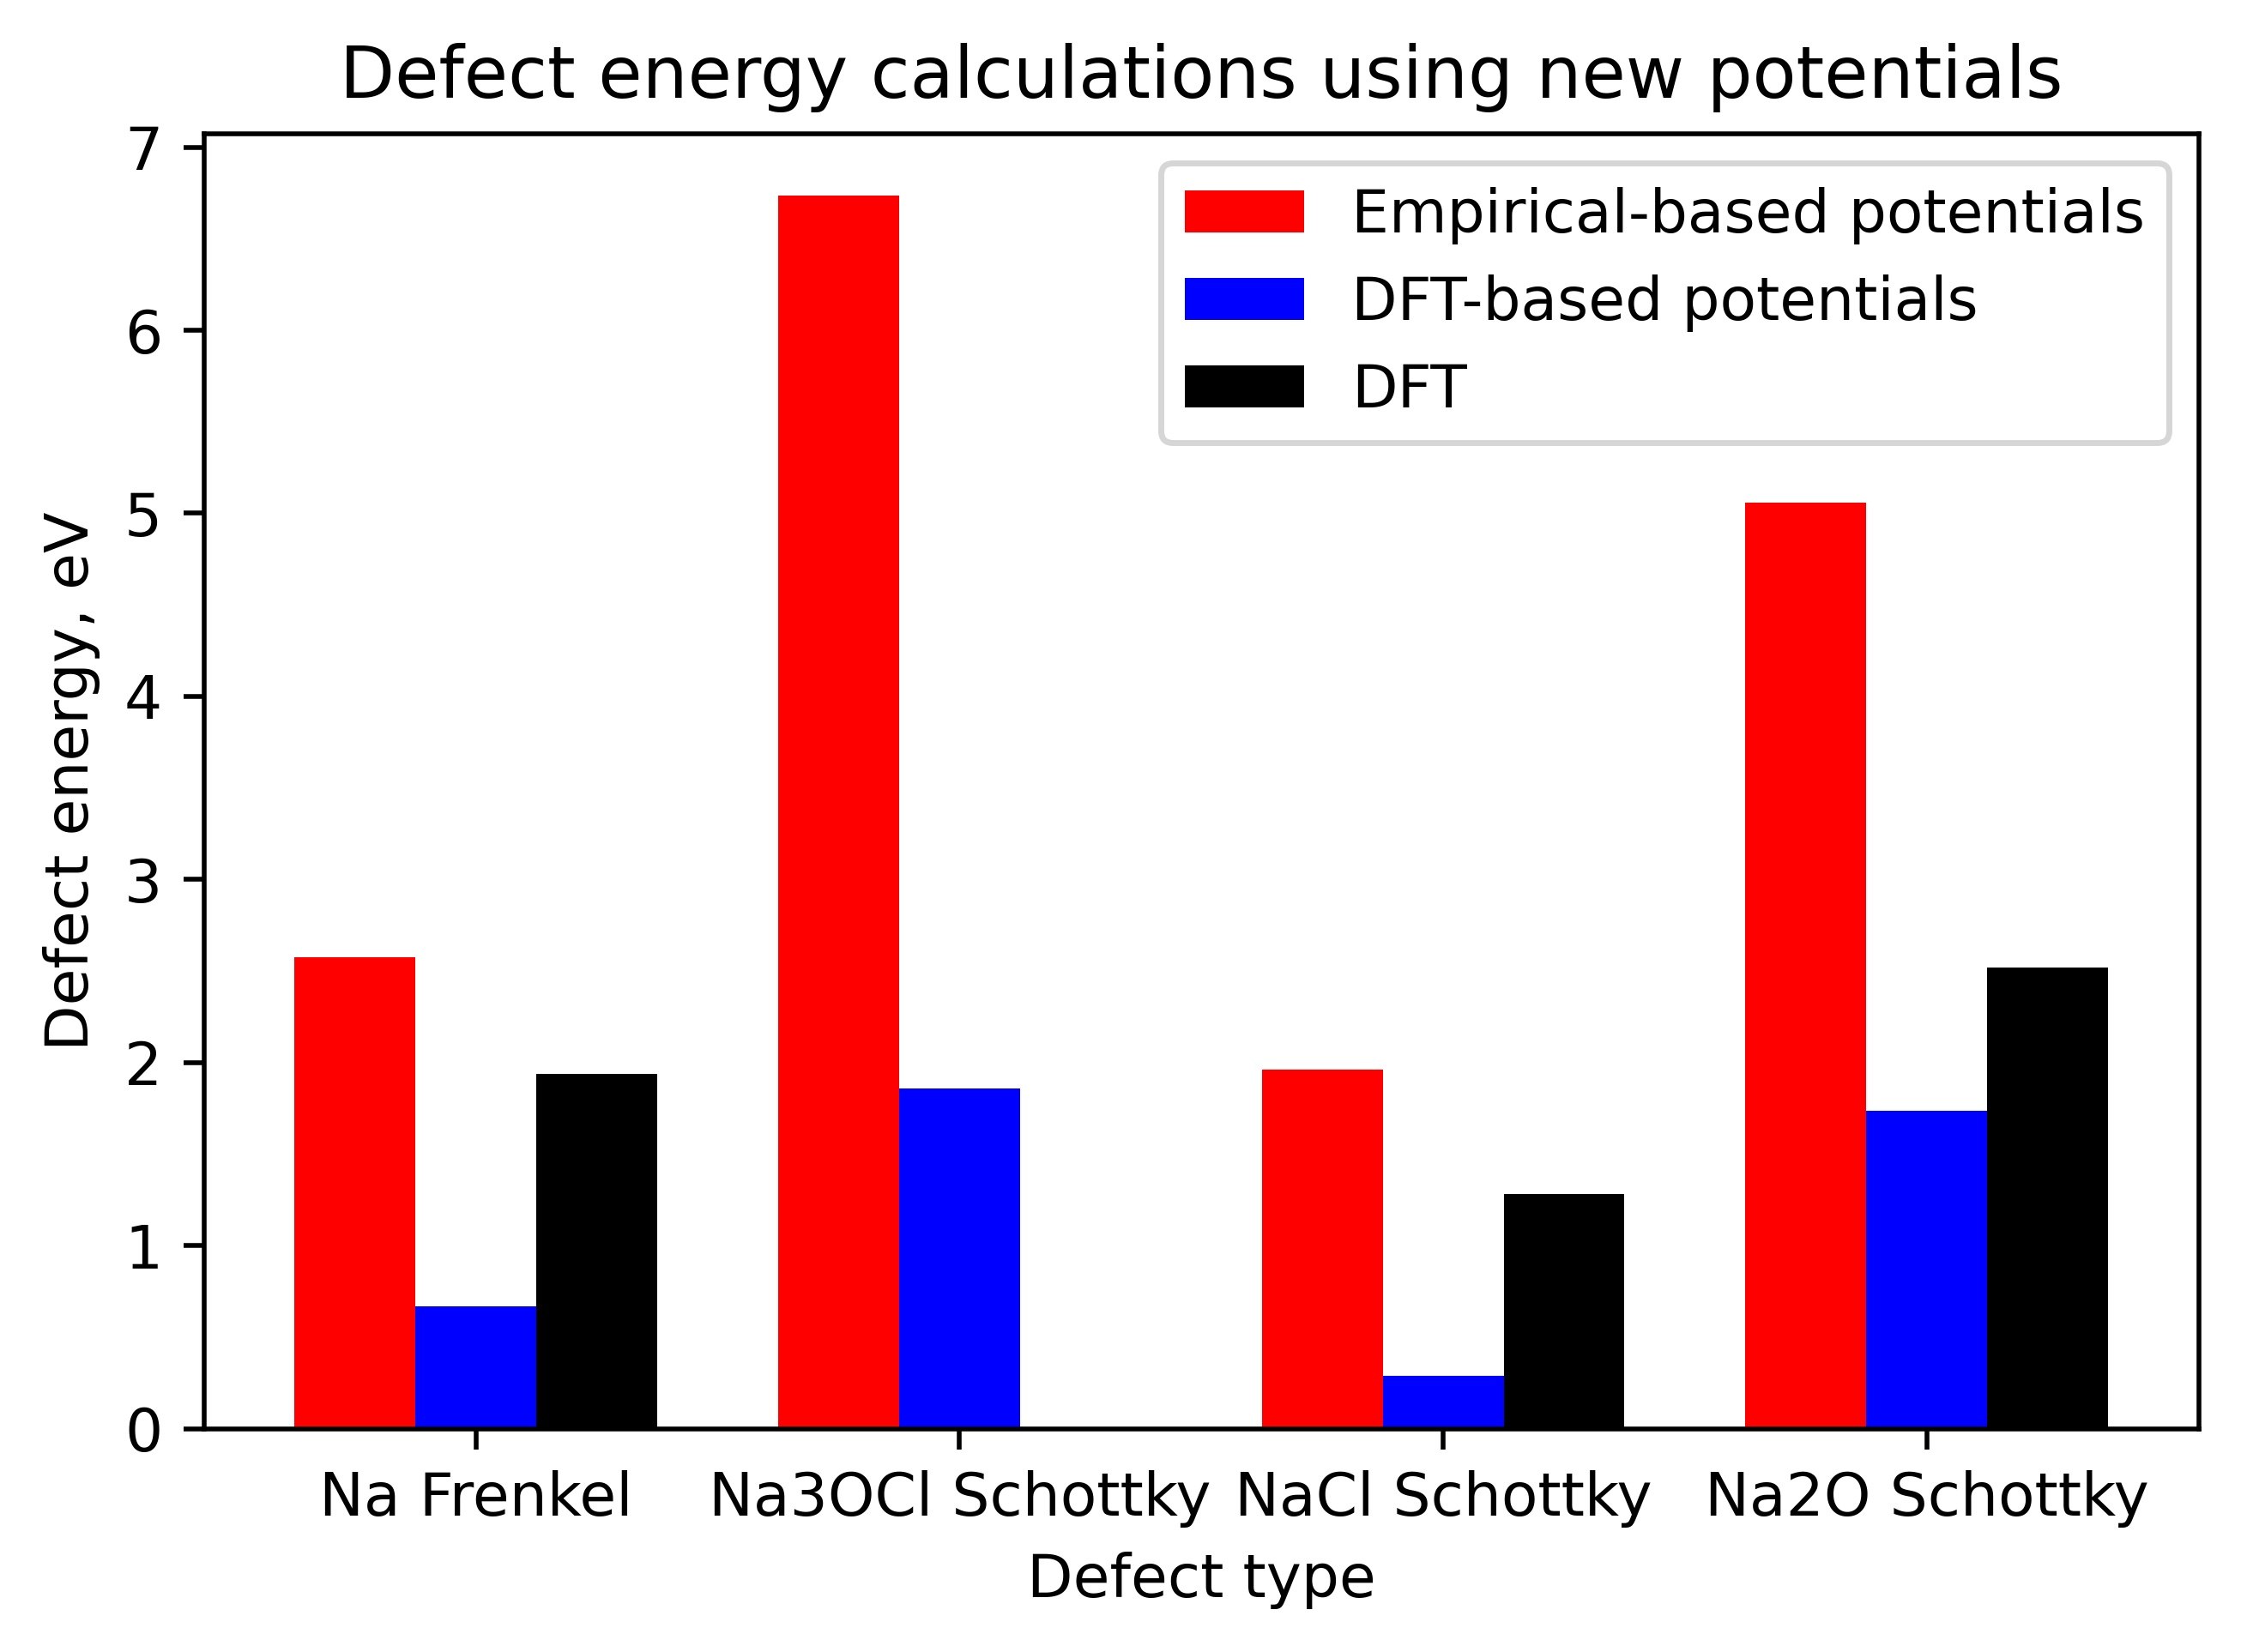
\includegraphics[width=0.45\textwidth]{lucy_defects.jpg}
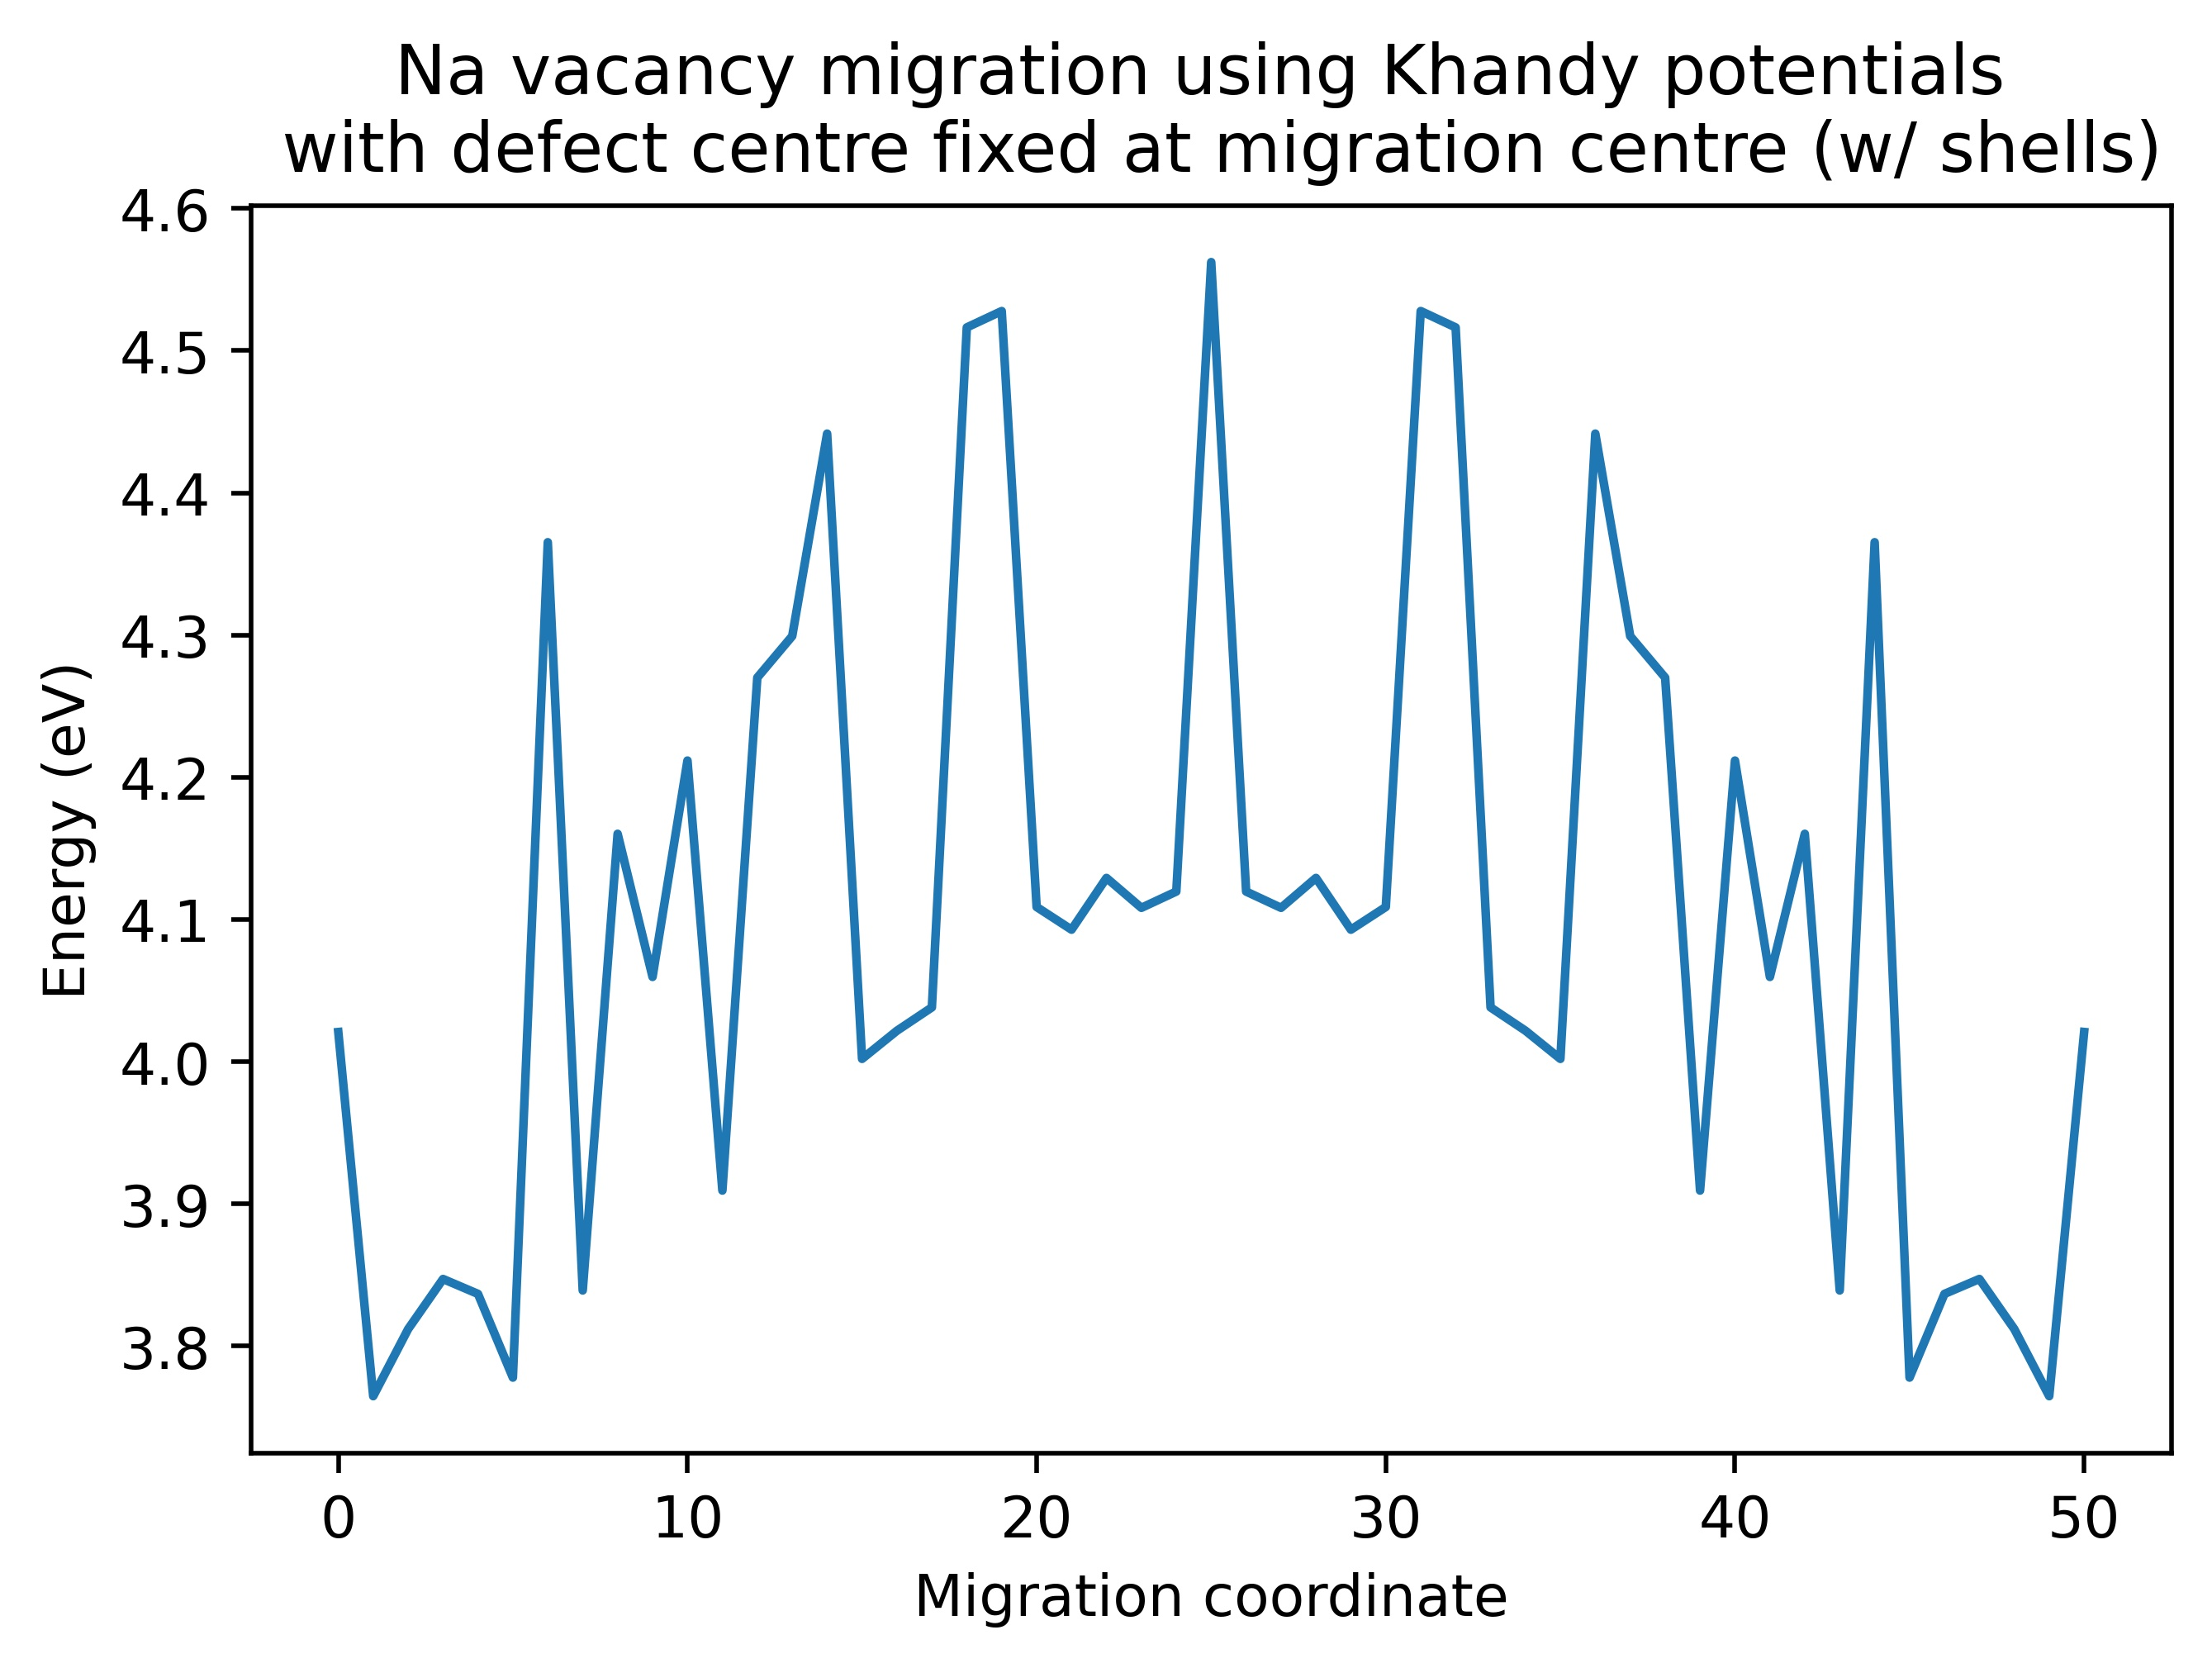
\includegraphics[width=0.45\textwidth]{lucy_migration.jpg}
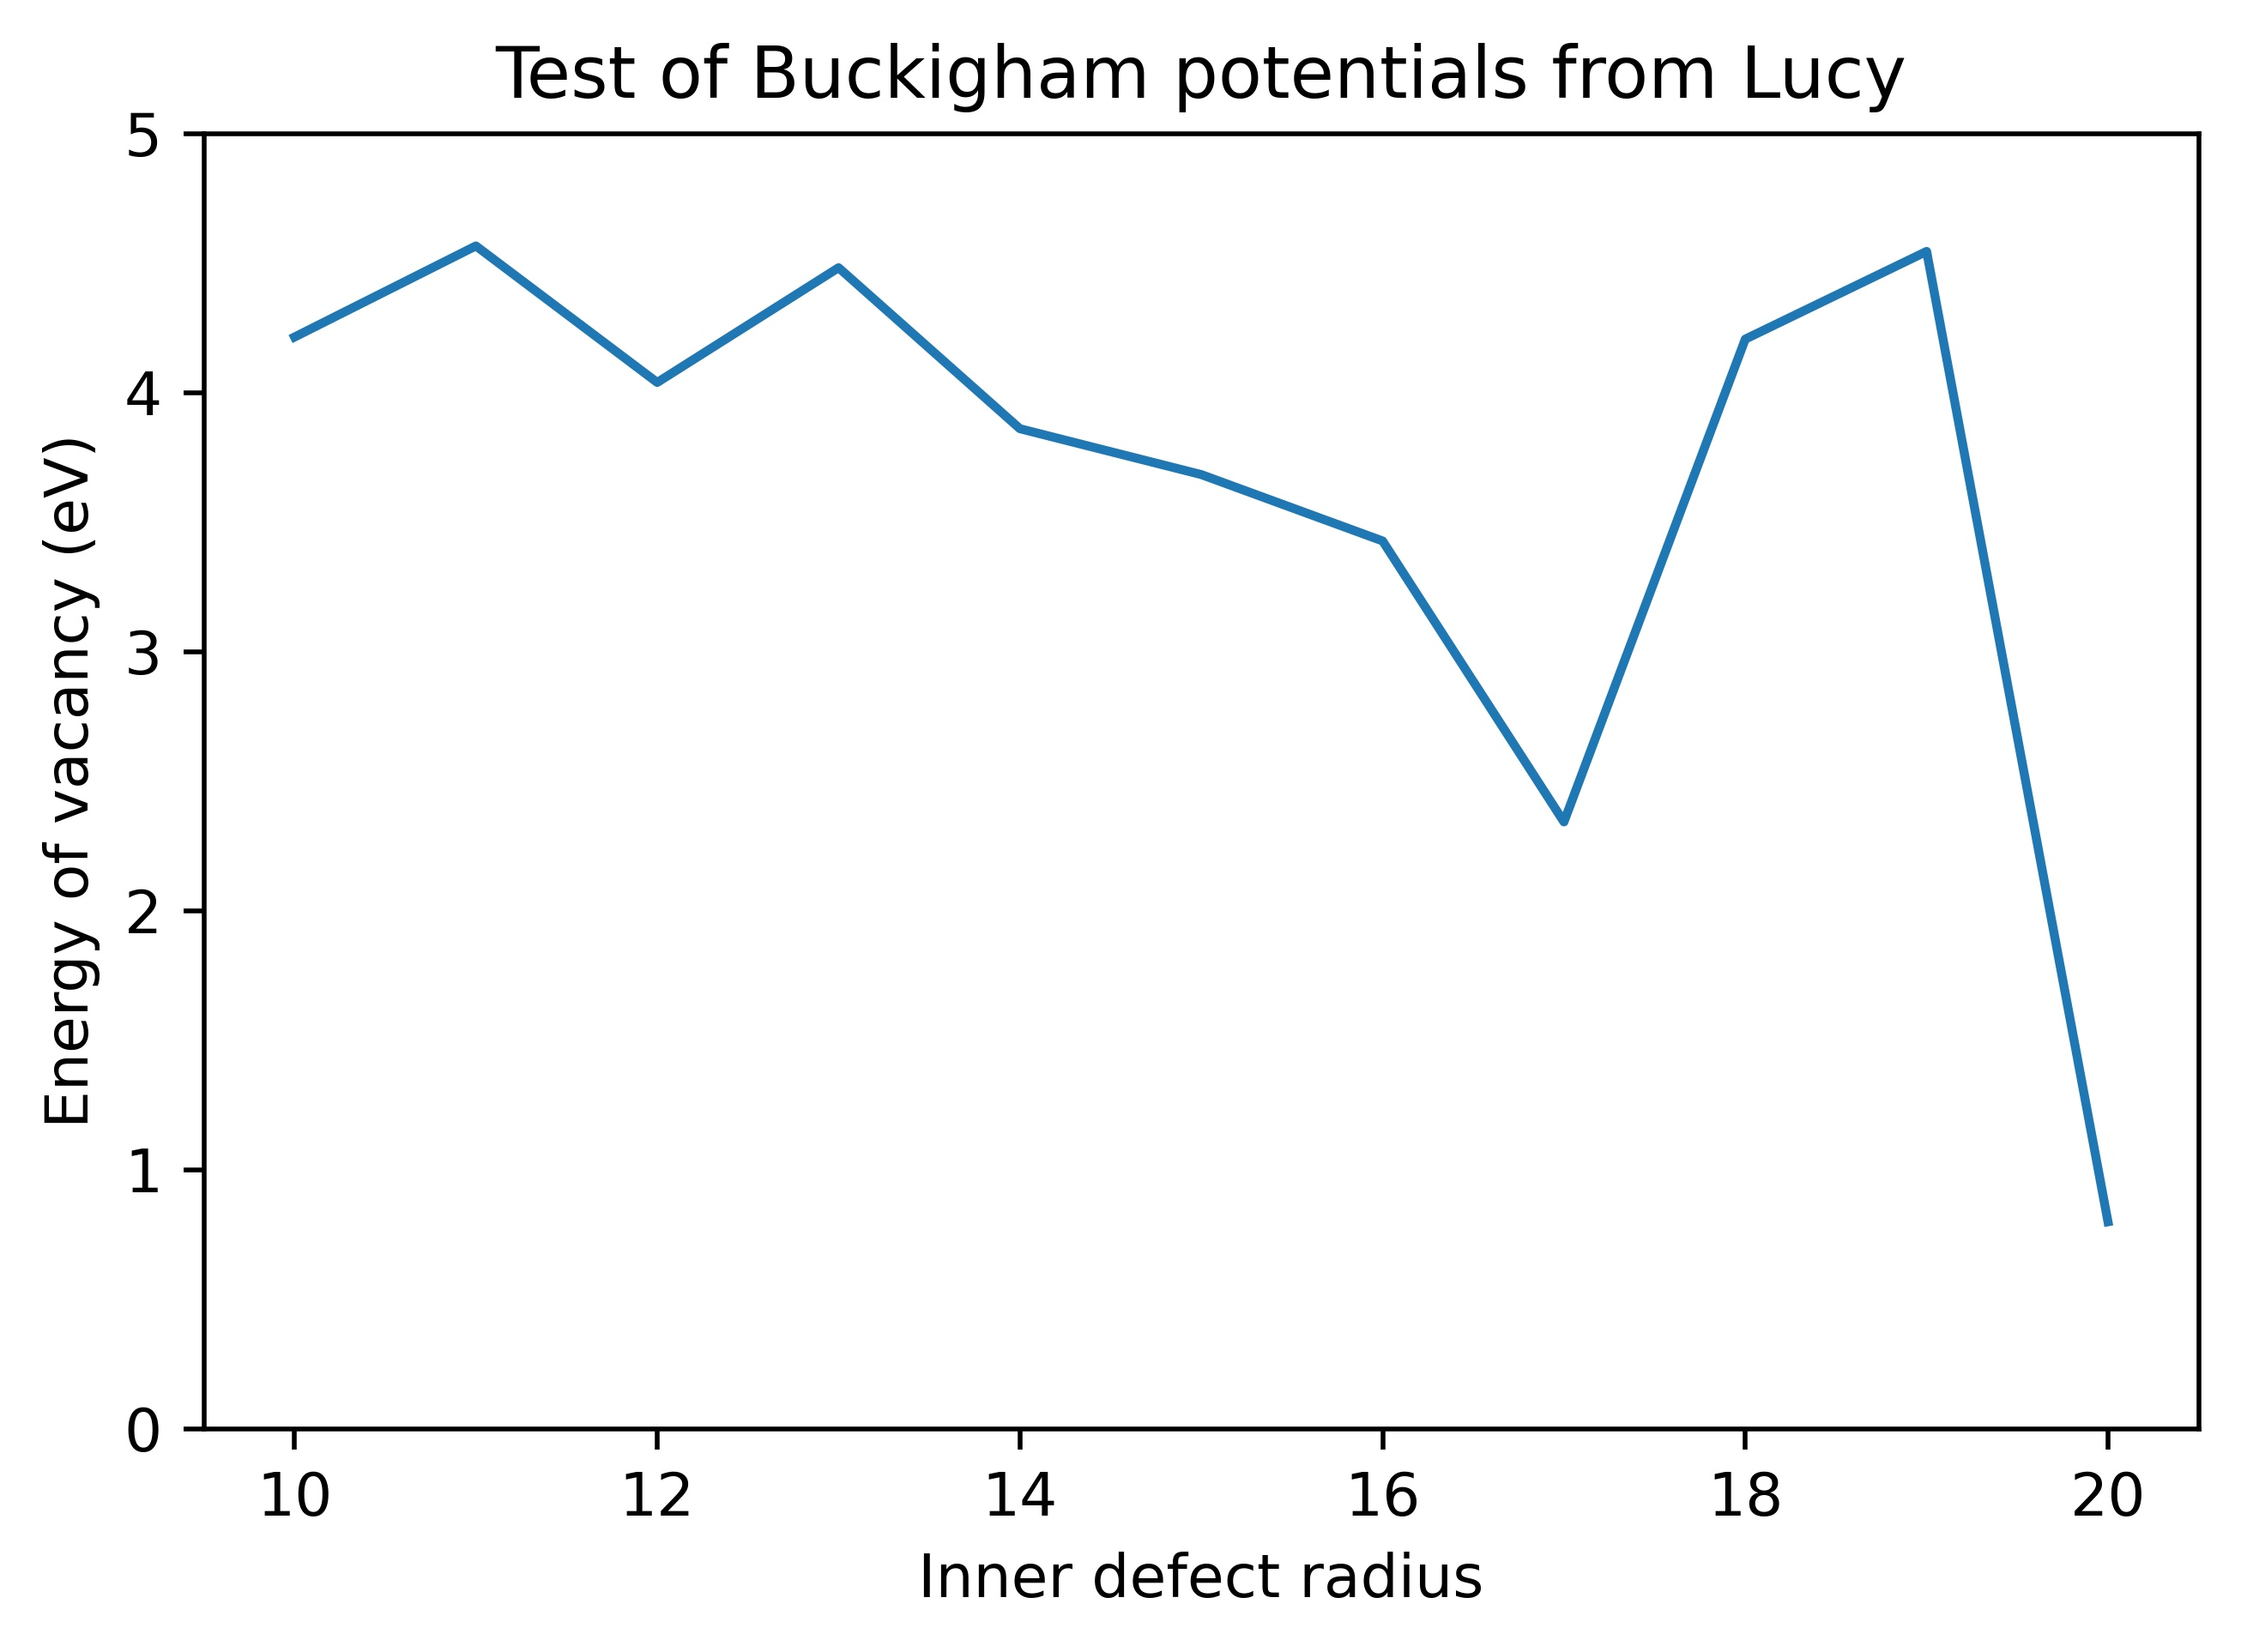
\includegraphics[width=0.45\textwidth]{lucy_test.jpg}
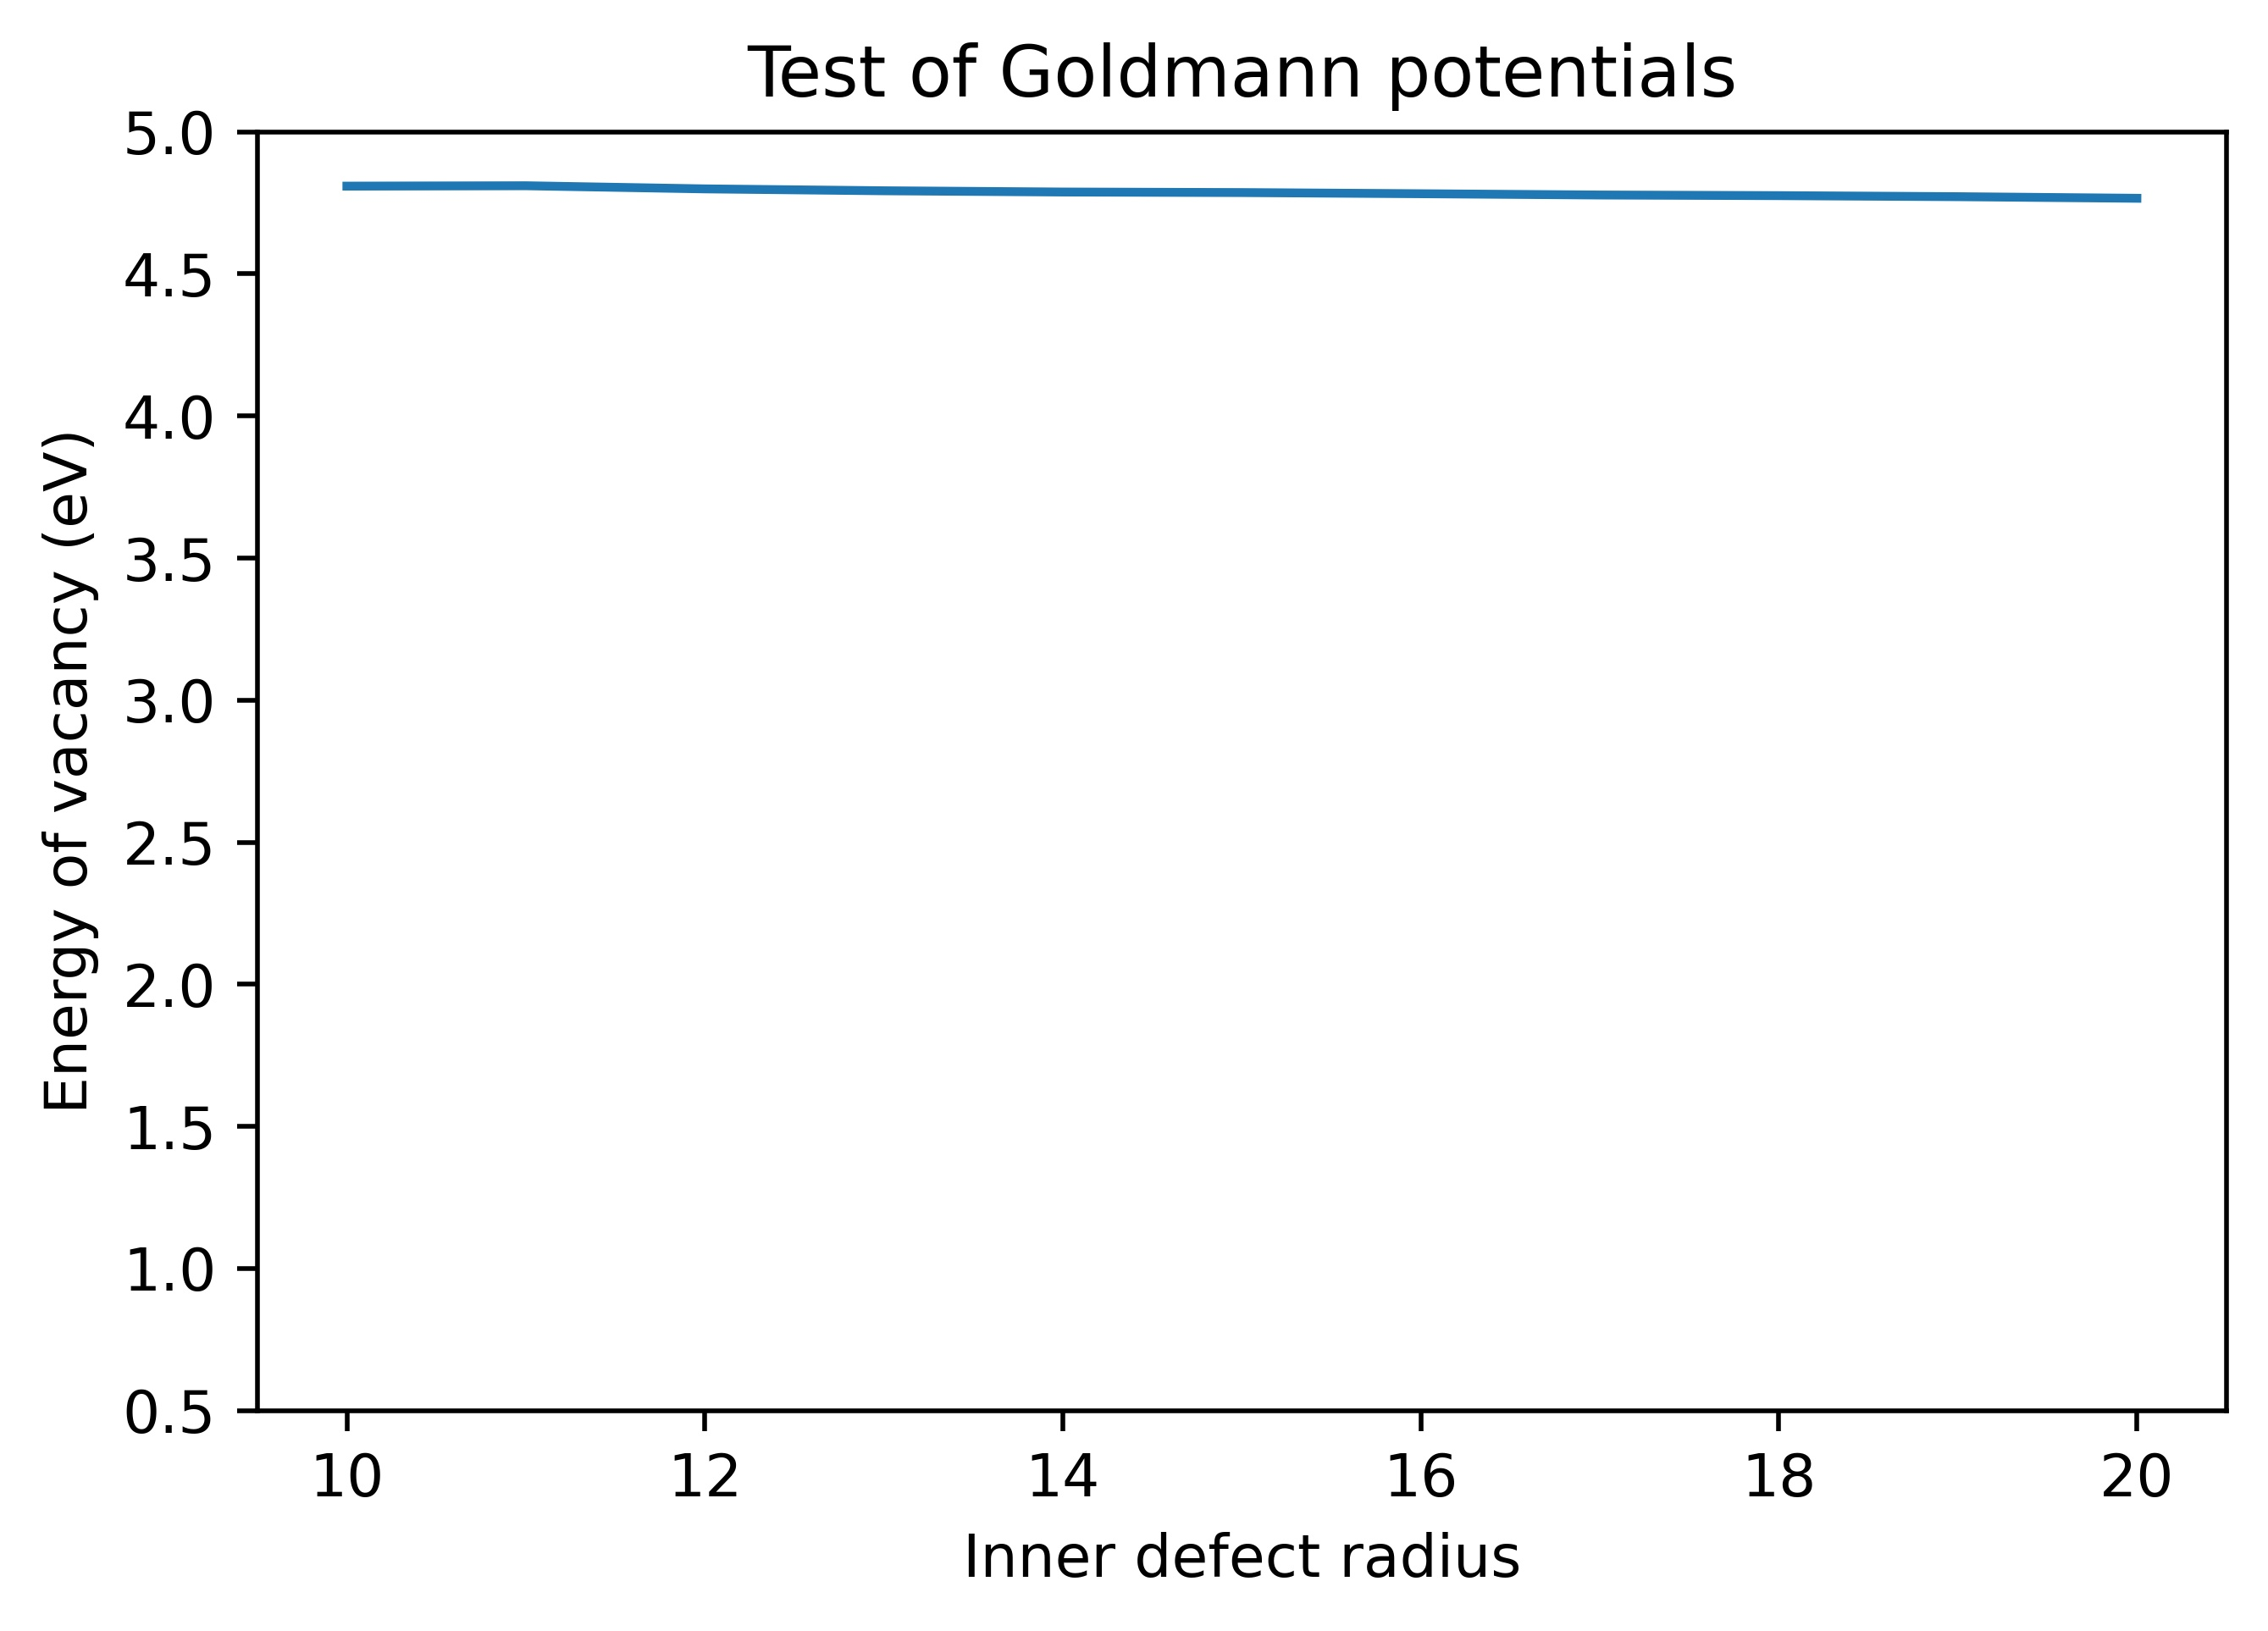
\includegraphics[width=0.45\textwidth]{khandy_test_scaled.jpg}
\end{figure}

\end{frame}

\begin{frame}
\frametitle{Initial MD calculations}

\begin{figure}
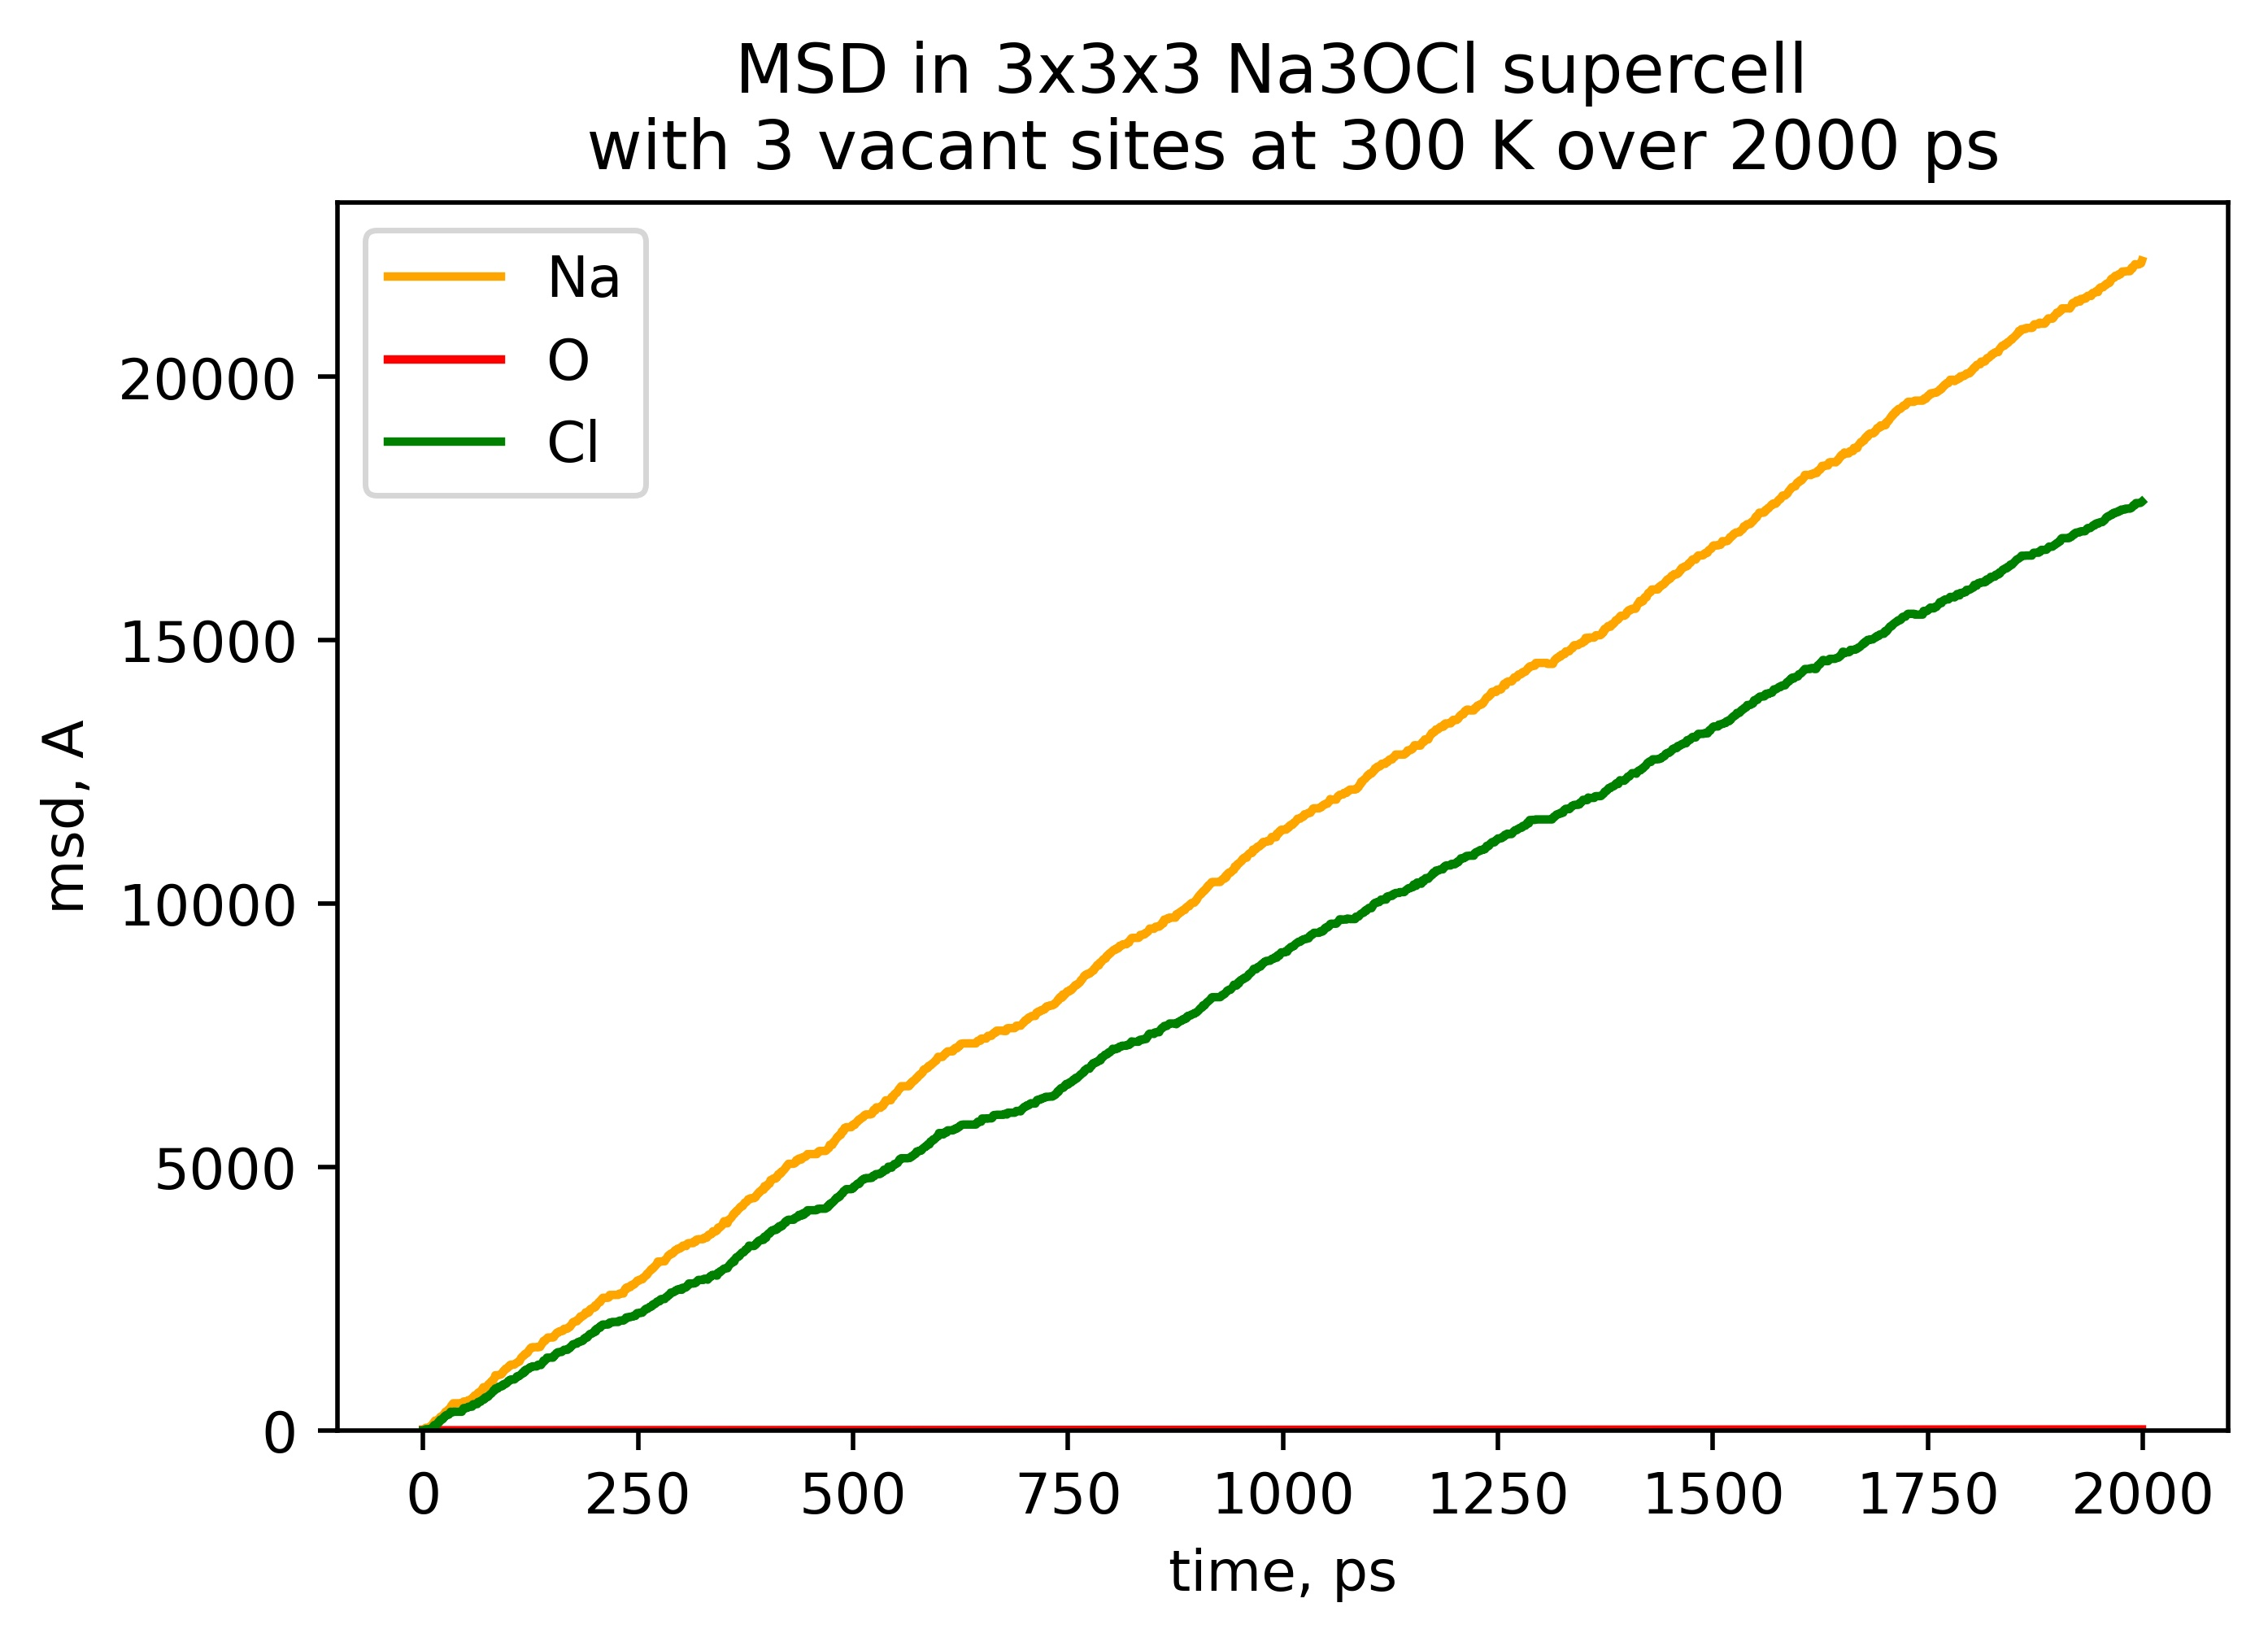
\includegraphics[width=0.45\textwidth]{3v_300k_msd.jpg}
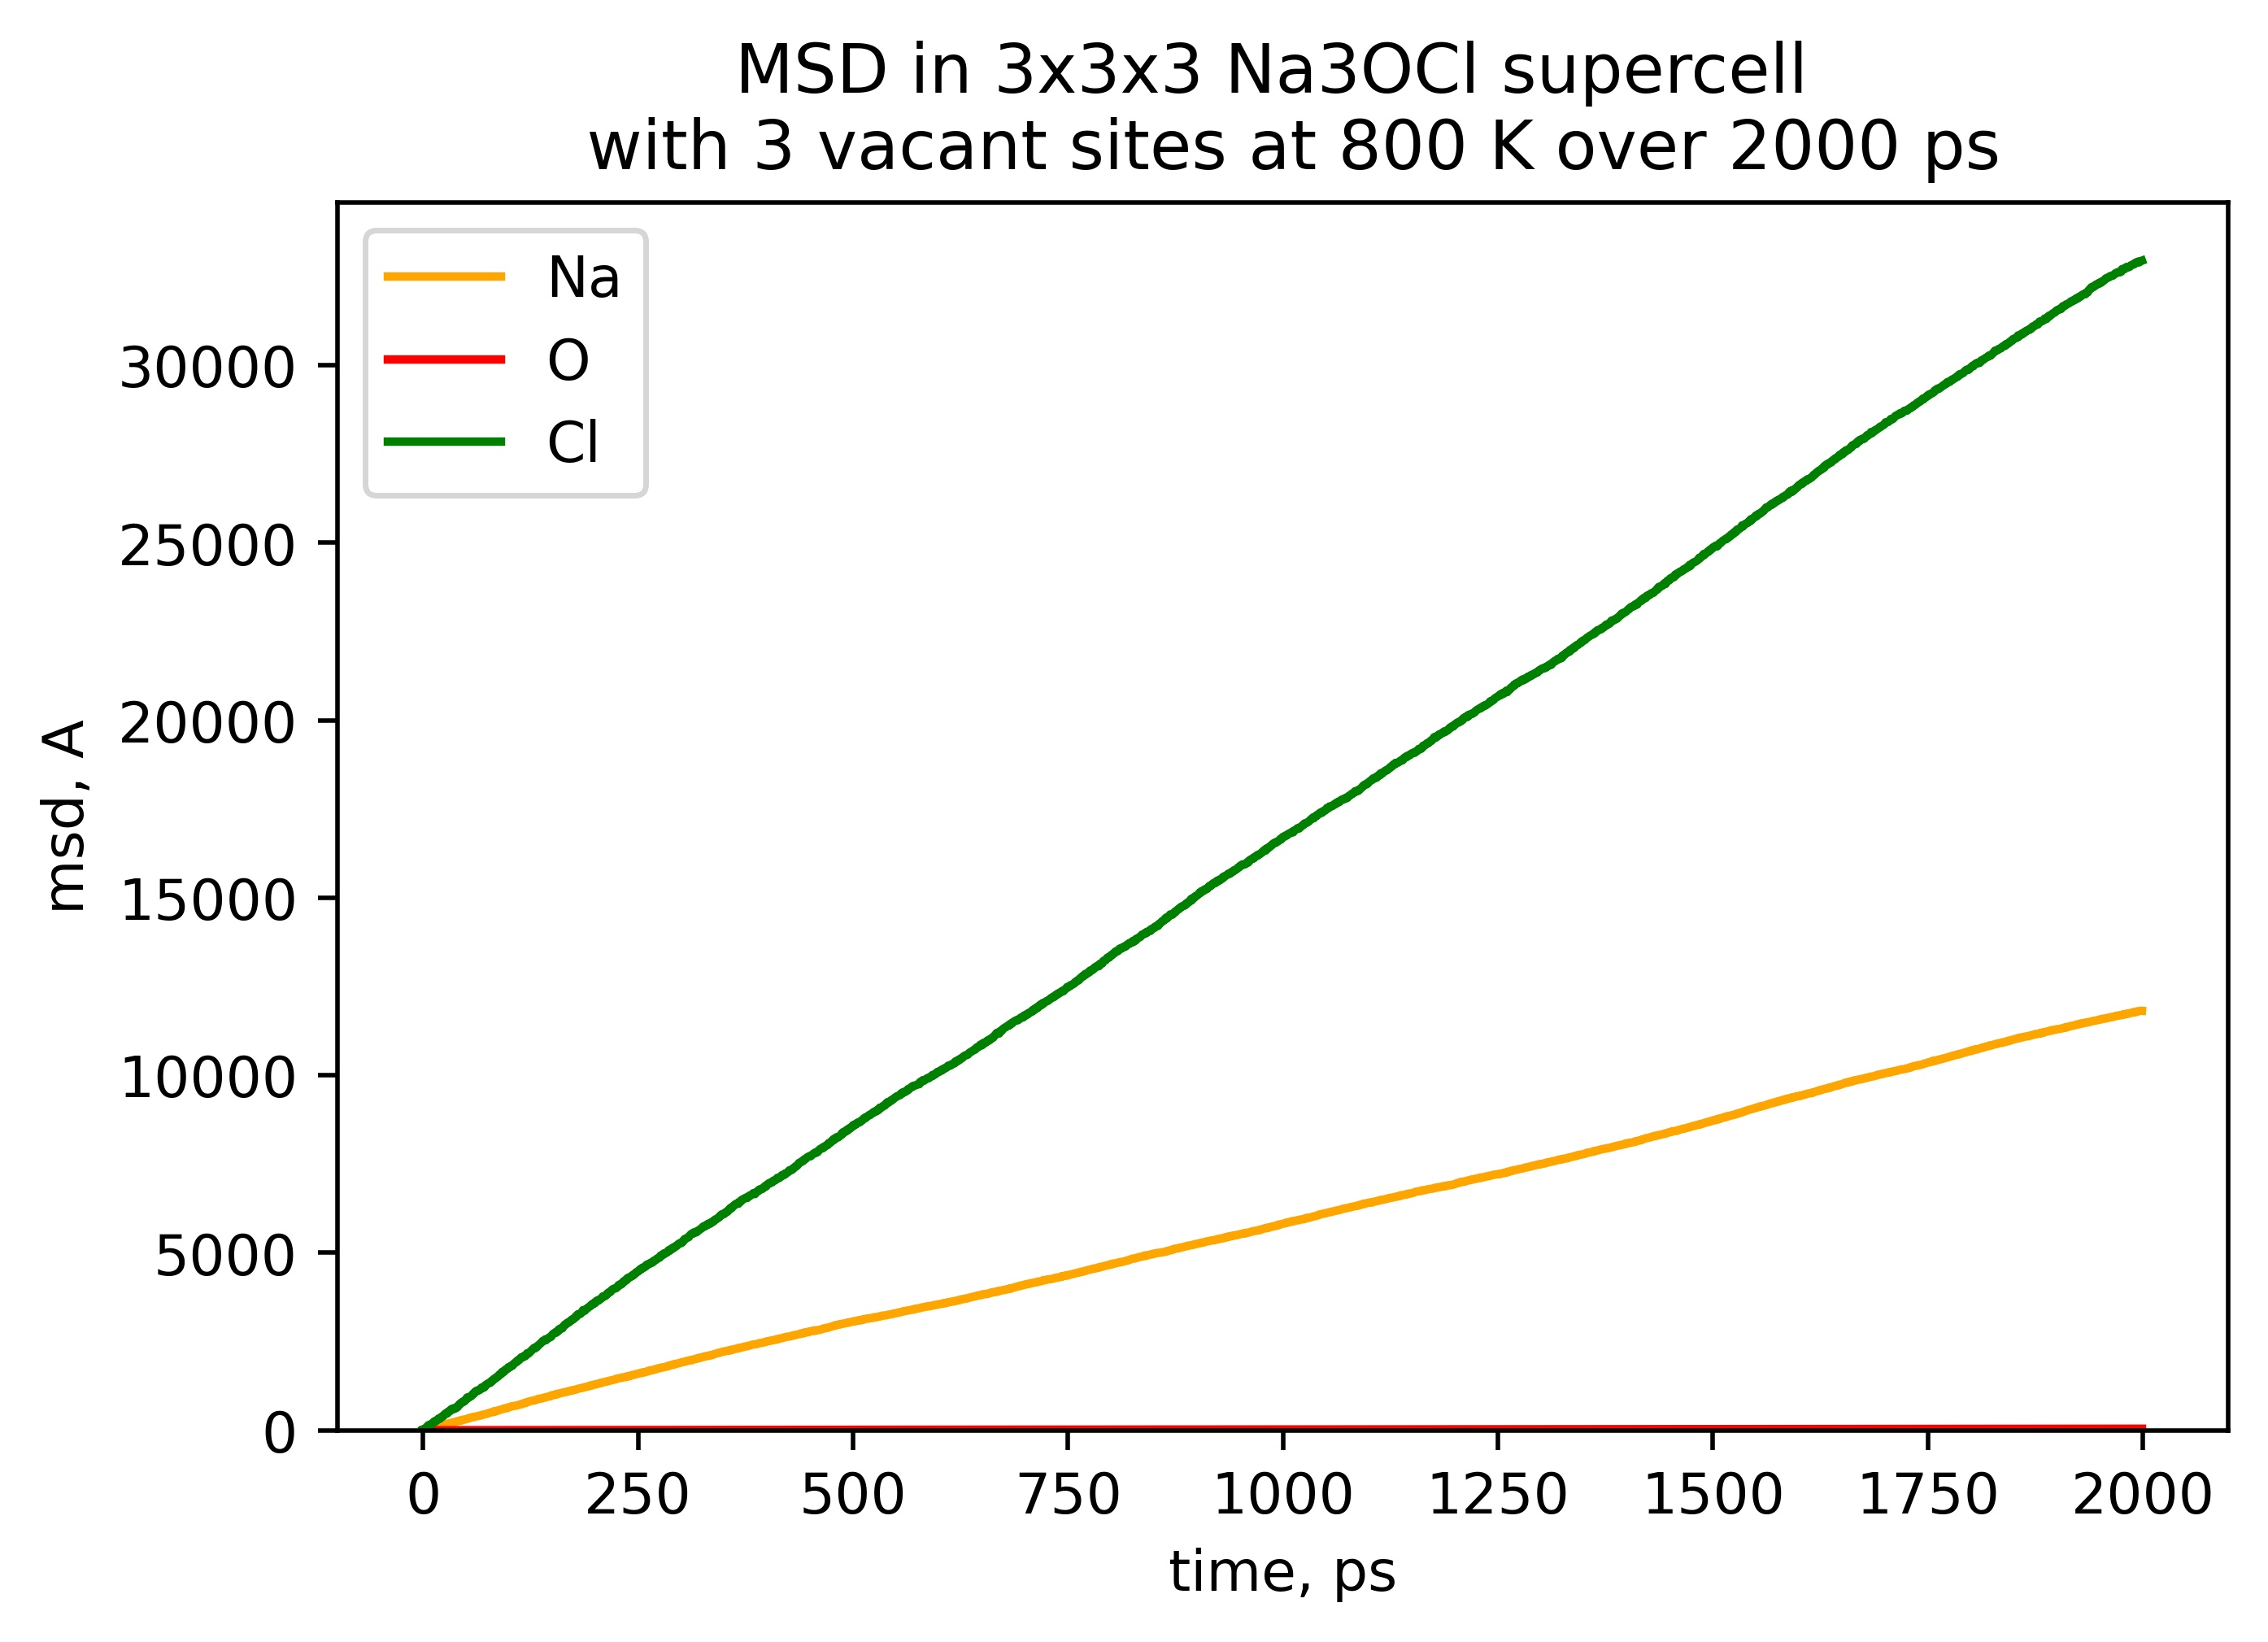
\includegraphics[width=0.45\textwidth]{3v_800k_msd.jpg}
\end{figure}

\end{frame}

\begin{frame}
\frametitle{2 ps run with 1 fs steps}

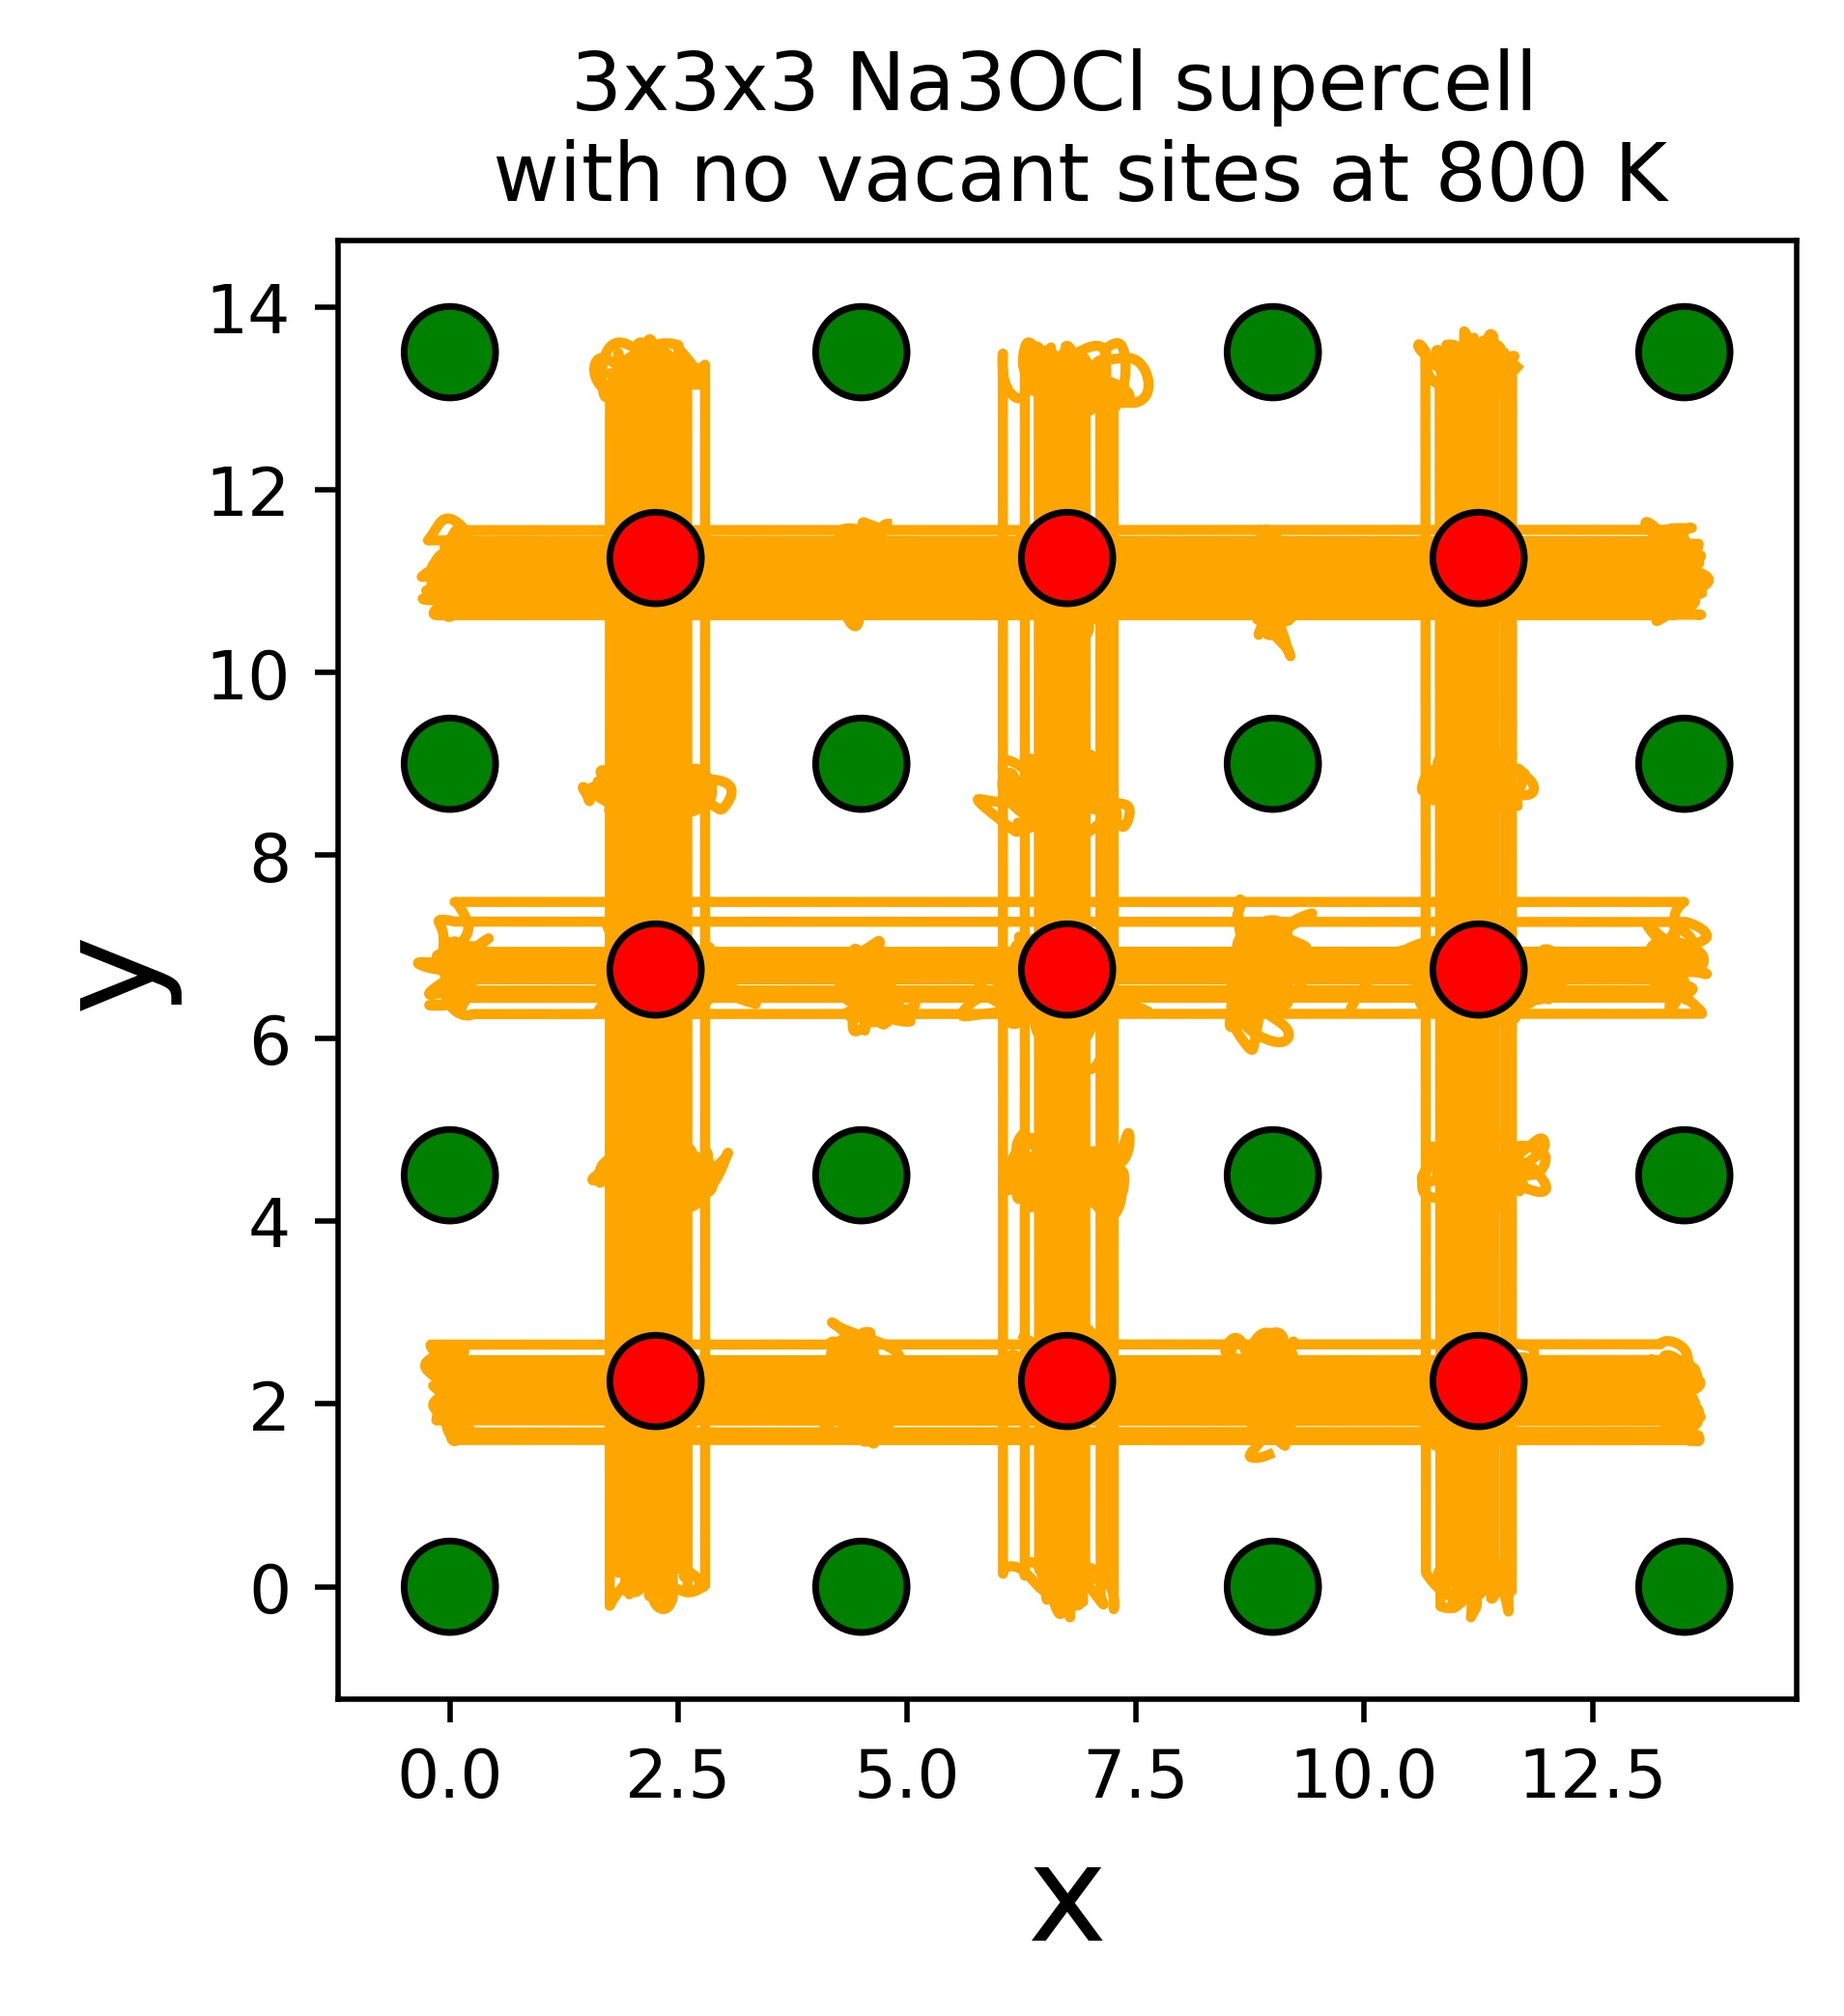
\includegraphics[width=0.2\textwidth]{800k_3v_xy.jpg}
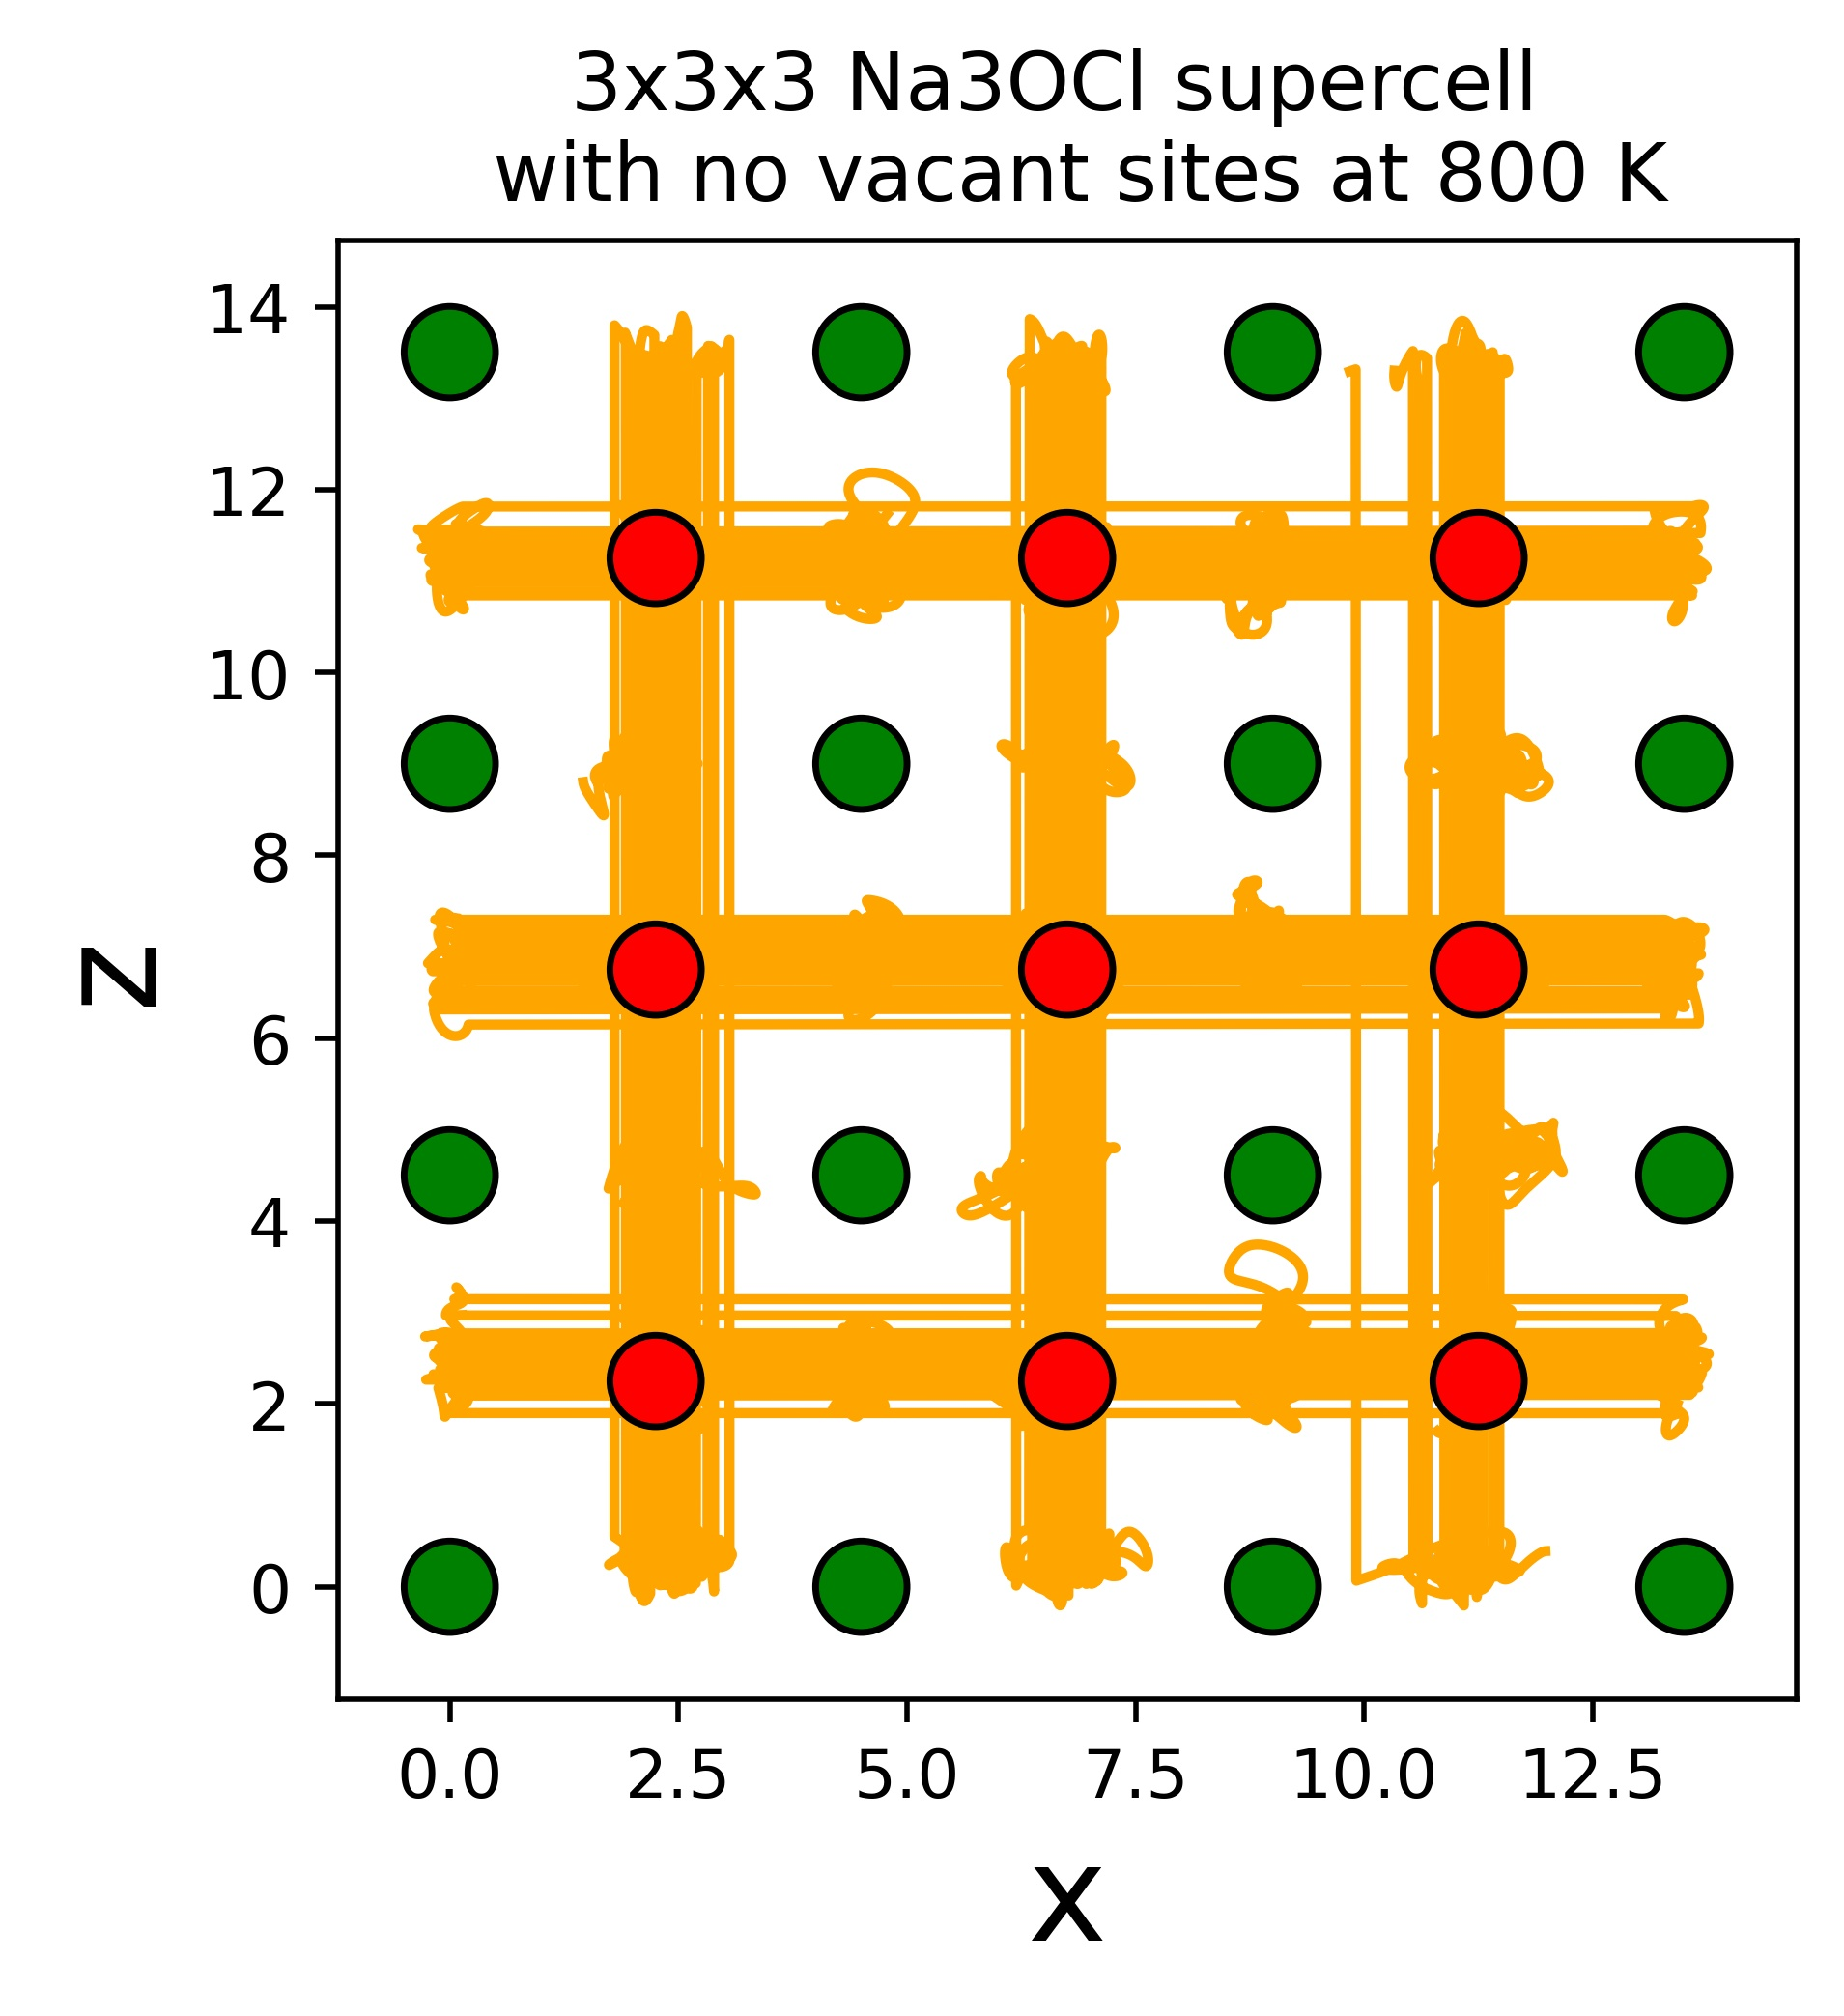
\includegraphics[width=0.2\textwidth]{800k_3v_xz.jpg}
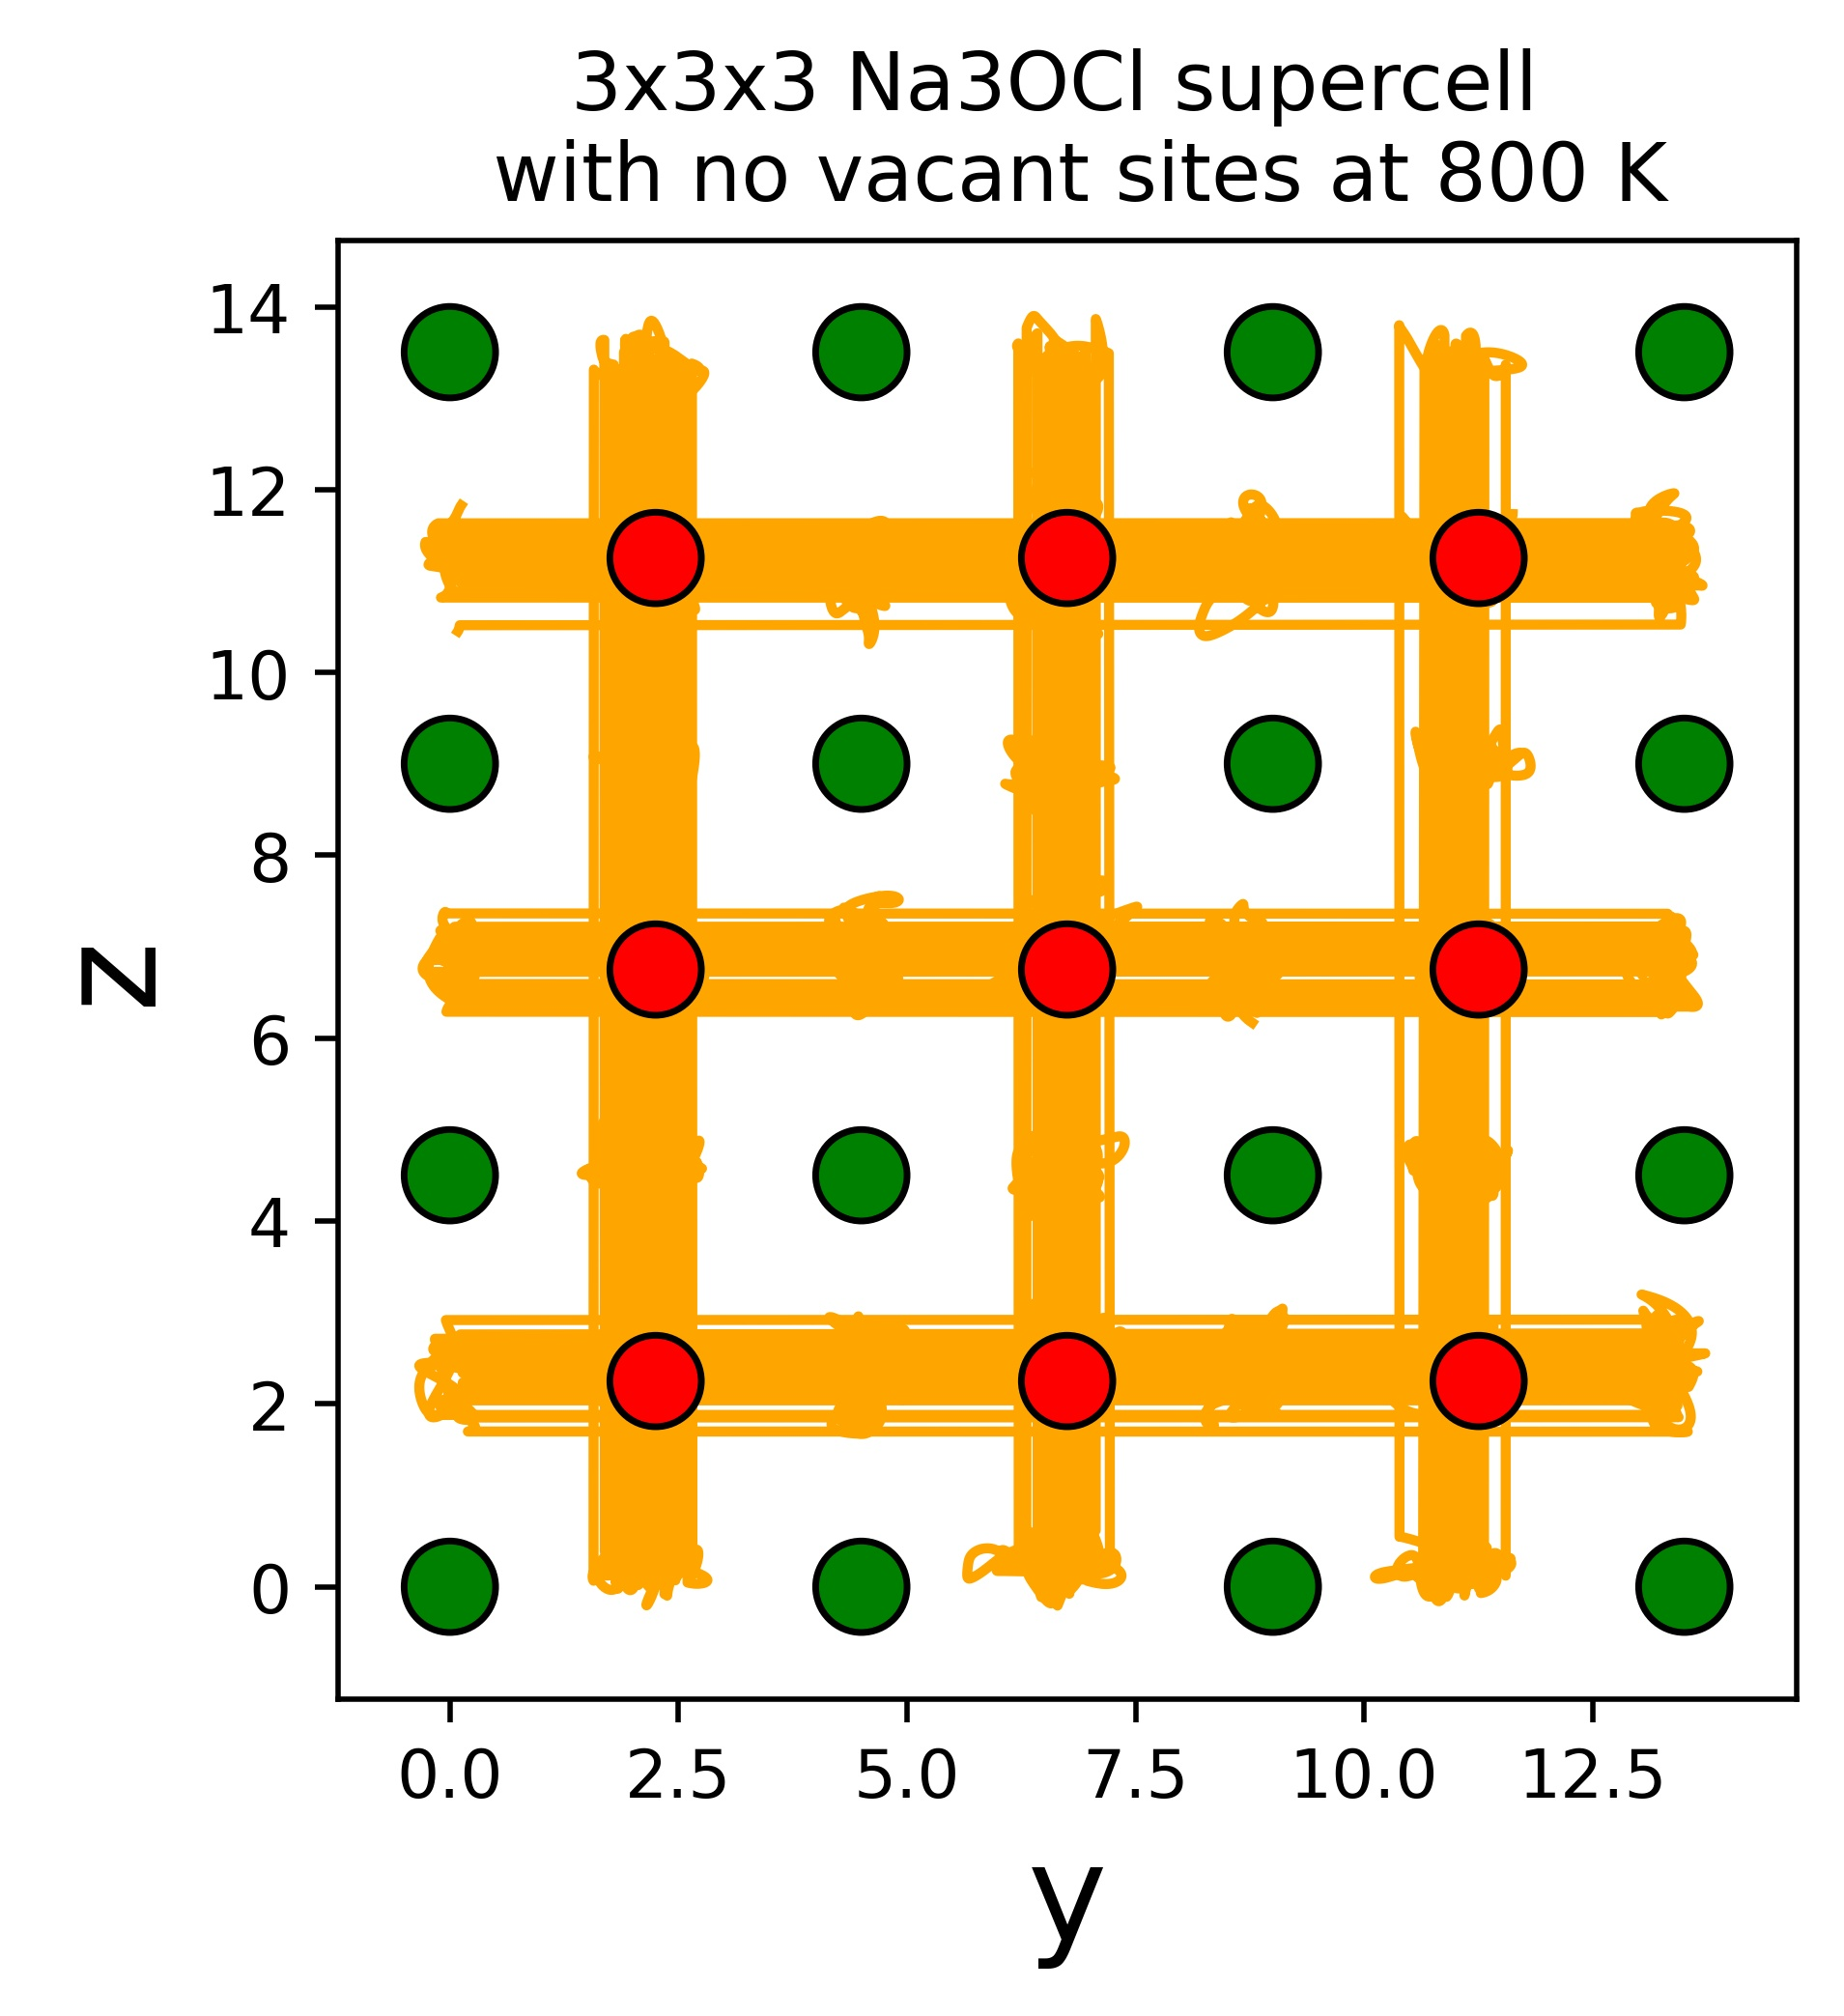
\includegraphics[width=0.2\textwidth]{800k_3v_yz.jpg}
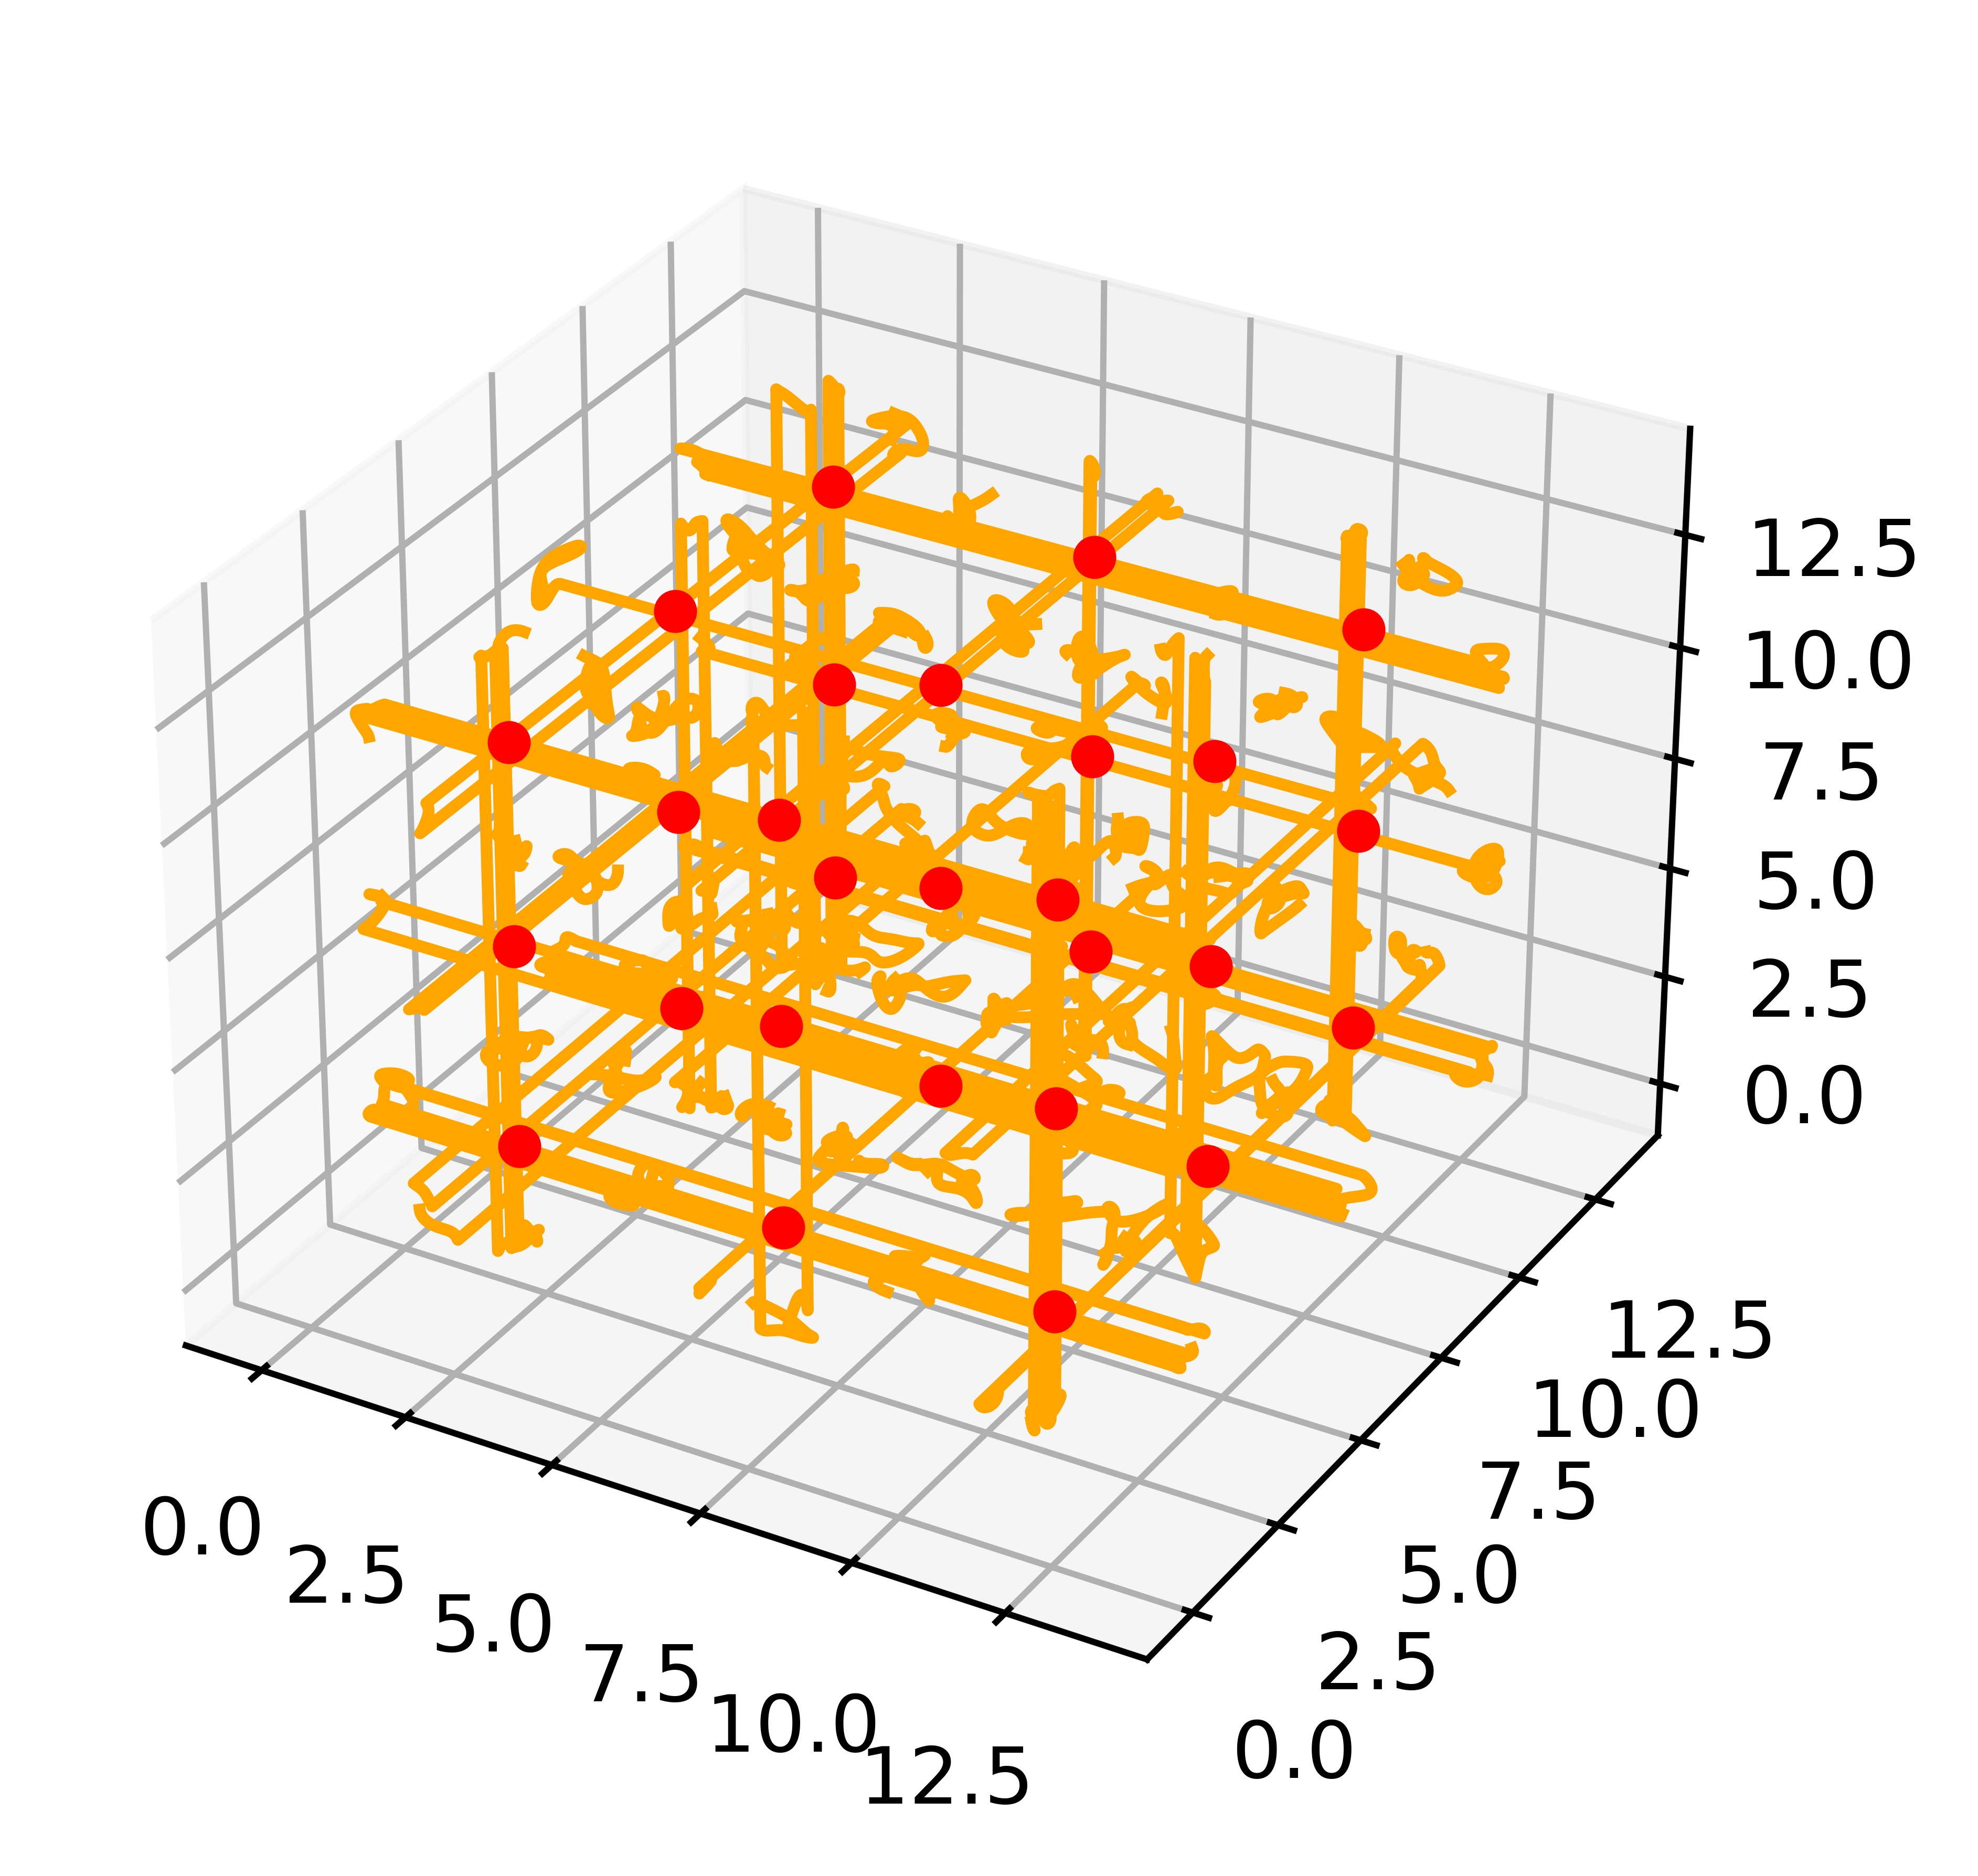
\includegraphics[width=0.25\textwidth]{800k_3v_3d.jpg}

\end{frame}

\end{document}